\chapter{\label{R_D}Results and Discussions}
The output separation of the signal and background after the training of the model are given in the \autoref{fig:three graphs}. These separation corresponds to the output with different level of separation. The level of separation are increasing from training in using Tprime[600-700 GeV] to  Tprime[1100-1200 GeV]. The training and testing accuracy can be seen in the \autoref{tab:my_label_table_1}.

\begin{figure}[H]
     \centering
     \begin{subfigure}[b]{0.47\textwidth}
         \centering
         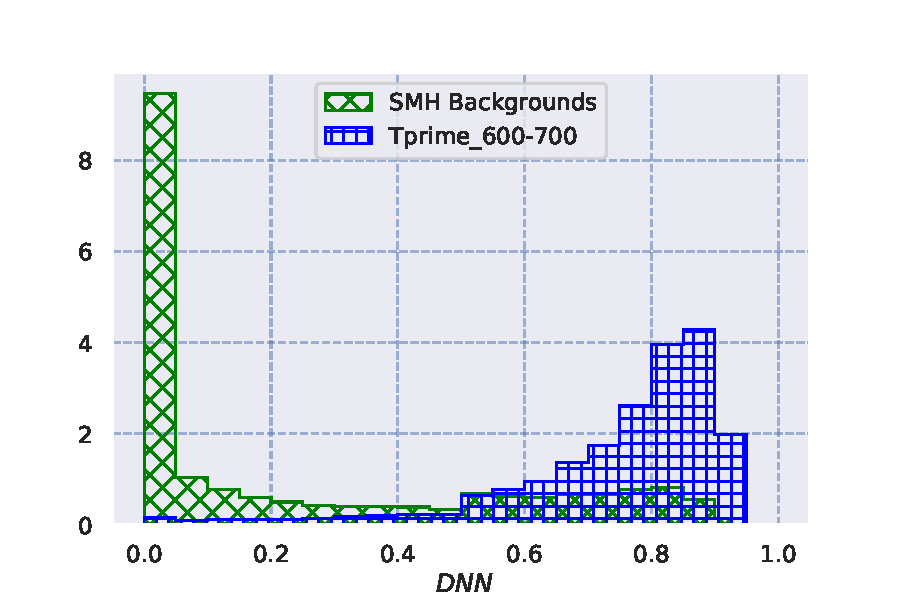
\includegraphics[width=\textwidth]{figure_4/output_TPrime600-700_on_testing_all_background.pdf}
         \caption{Tprime(600-700GeV)}
         \label{fig:y equals x}
     \end{subfigure}
     \hfill
     \begin{subfigure}[b]{0.47\textwidth}
         \centering
         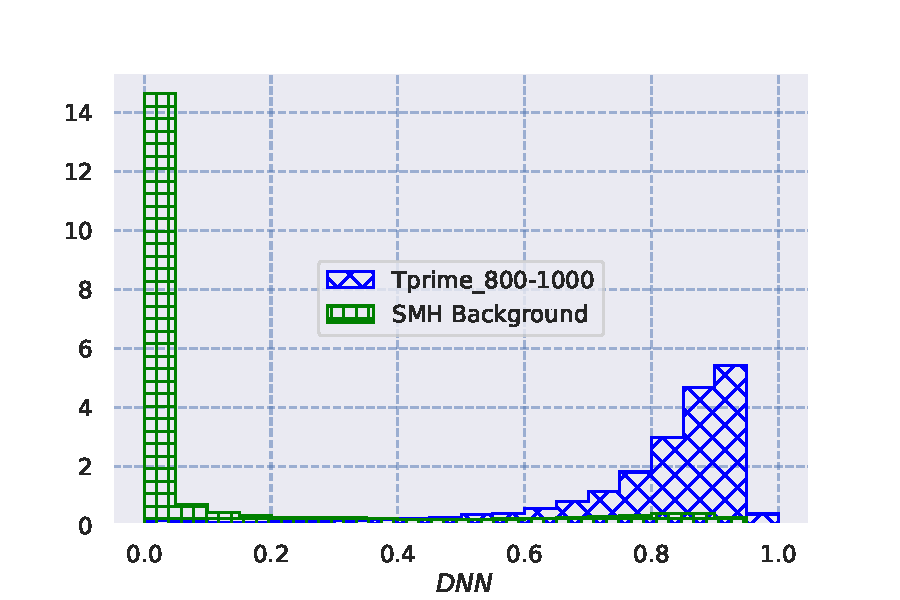
\includegraphics[width=\textwidth]{figure_4/output_TPrime800-1000_on_testing_all_background.pdf}
         \caption{Tprime(800-1000GeV)}
         \label{fig:three sin x}
     \end{subfigure}
     \hfill
     \begin{subfigure}[b]{0.47\textwidth}
         \centering
         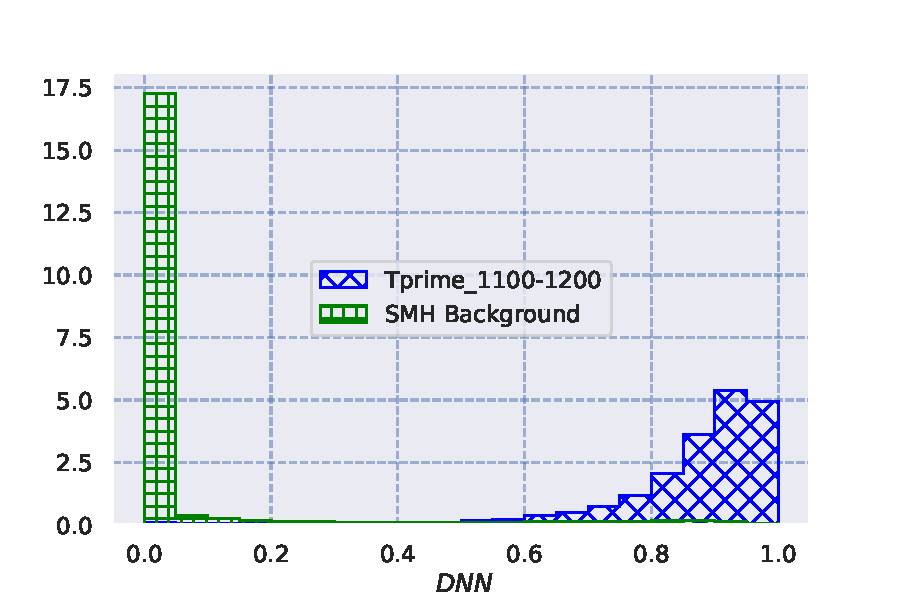
\includegraphics[width=\textwidth]{figure_4/Training_with_Tprime_1100-1200GeV_ with_backgrounds.pdf}
         \caption{Tprime(1100-1200GeV)}
         \label{fig:five over x}
     \end{subfigure}
        \caption{Separation output of signal from the background after all different training }
        \label{fig:three graphs}
\end{figure}



% \section{Output from signal and background training}





\begin{table}[H]
    \centering
    \begin{tabular}{|c|c|c|}\hline
    Model     & Training   & Testing  \\
              & Accuracy (\%)  &     Accuracy (\%)  \\\hline
   Tprime[600-700GeV]       &     82.29        &    81.81         \\
   Tprime[800-1000GeV]          &   89.62          &     89.25        \\
   Tprime[1100-1200GeV]          &     94.76        &    94.37         \\
   Tprime[600-1200GeV]          &       87.32      &        87.14     \\\hline
    \end{tabular}
    \caption{Table with training and testing accuracy for the different training and testing with the standard model Higgs background. The output is increasing with the increase in the mass of Tprime from 600-1200GeV.}
    \label{tab:my_label_table_1}
\end{table}




The Receiving operator characteristic(ROC) curve for the different training from Tprime[600-700], Tprime[800-1000], and Tprime[1100-1200] can be compared with the \autoref{fig:my_label_ROC}. The ROC curve suggest the correlation between the signal and background efficiencies. This helps for the background rejections. 
\begin{figure}[H]
    \centering
    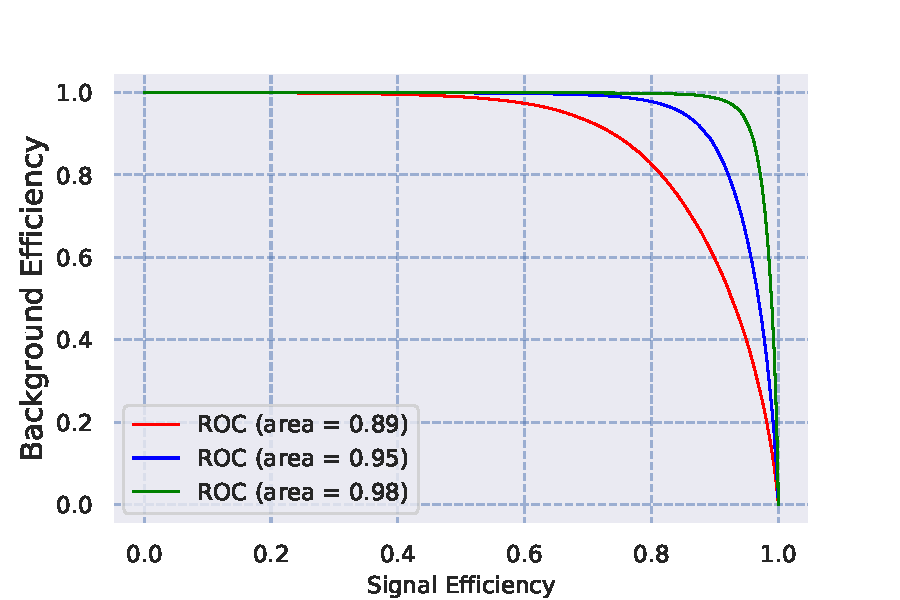
\includegraphics{Results_outputs/ROC_curve_Comaprision_Different_training.pdf}
    \caption{ Receiving operator characteristic(ROC) curve for all the different training and testing output. The ROC area under the curve increasing with the increasing in the training of the mass point.}
    \label{fig:my_label_ROC}
\end{figure}


The output after testing on the DNN score from the different training are represented as in the form of stacked ratio plot as in \autoref{fig:stacked_plot_DNN_100}. All the output are from different training output after testing on standard model Higgs (SMH) backgrounds, Non-resonant backgrounds (NRBs) and on the signals corresponding to the training. The output plotted with applying the diphoton cut on  the monte carlo(MC) of the NRB and SMH, along with the datafile. The monte carlo have been scaled with the datafile as $\frac{Datafile}{MonteCarlo}$, which have been plotted as the ratio plot below the stacked histogram.\\

\begin{figure}[H]
     \centering
     \begin{subfigure}[b]{0.3\textwidth}
         \centering
         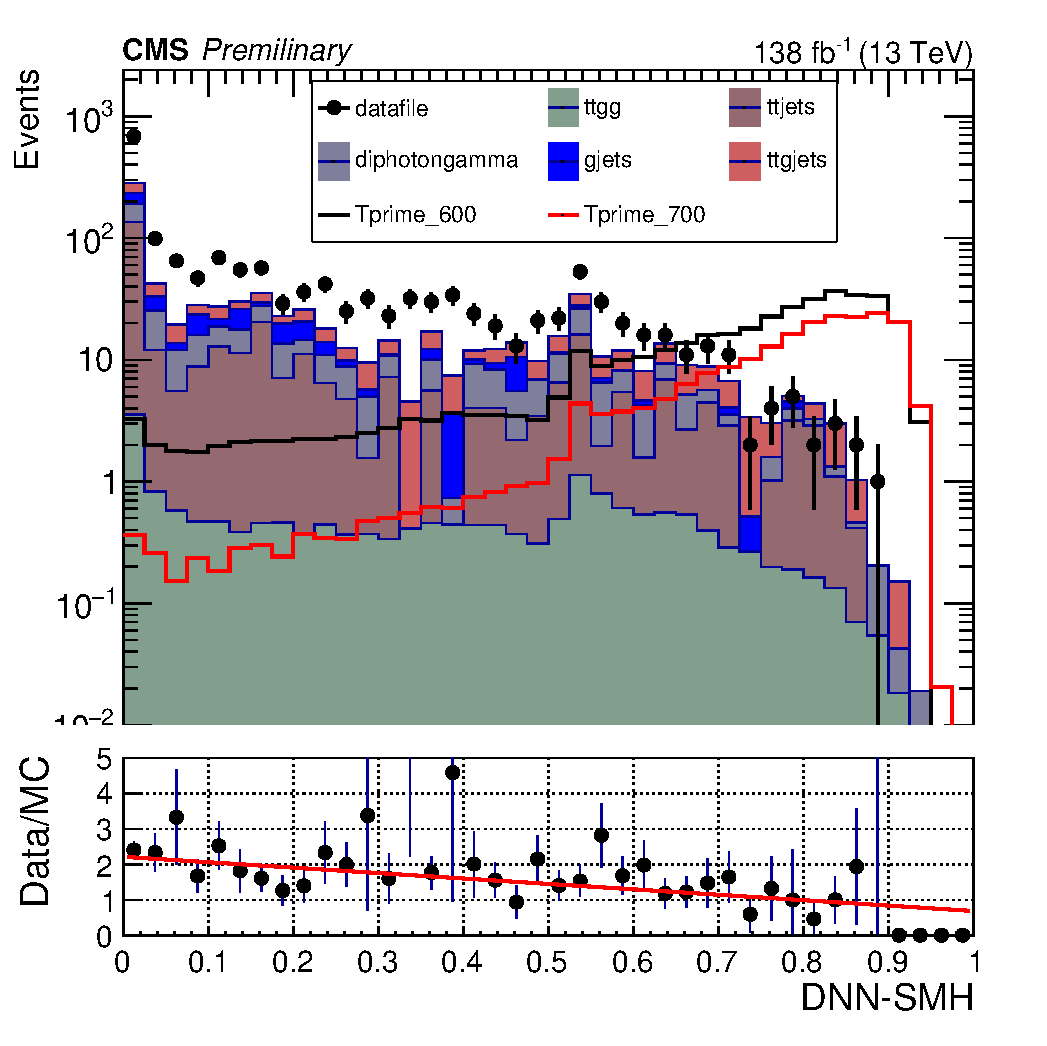
\includegraphics[width=\textwidth, scale = 0.5 ]{figure_4/Stacked_plot_DNN_600-700_with_diphoton_cuts.pdf}
        %  \caption{$y=x$}
        %  \label{fig:y equals x}
     \end{subfigure}
     \hfill
     \begin{subfigure}[b]{0.3\textwidth}
         \centering
         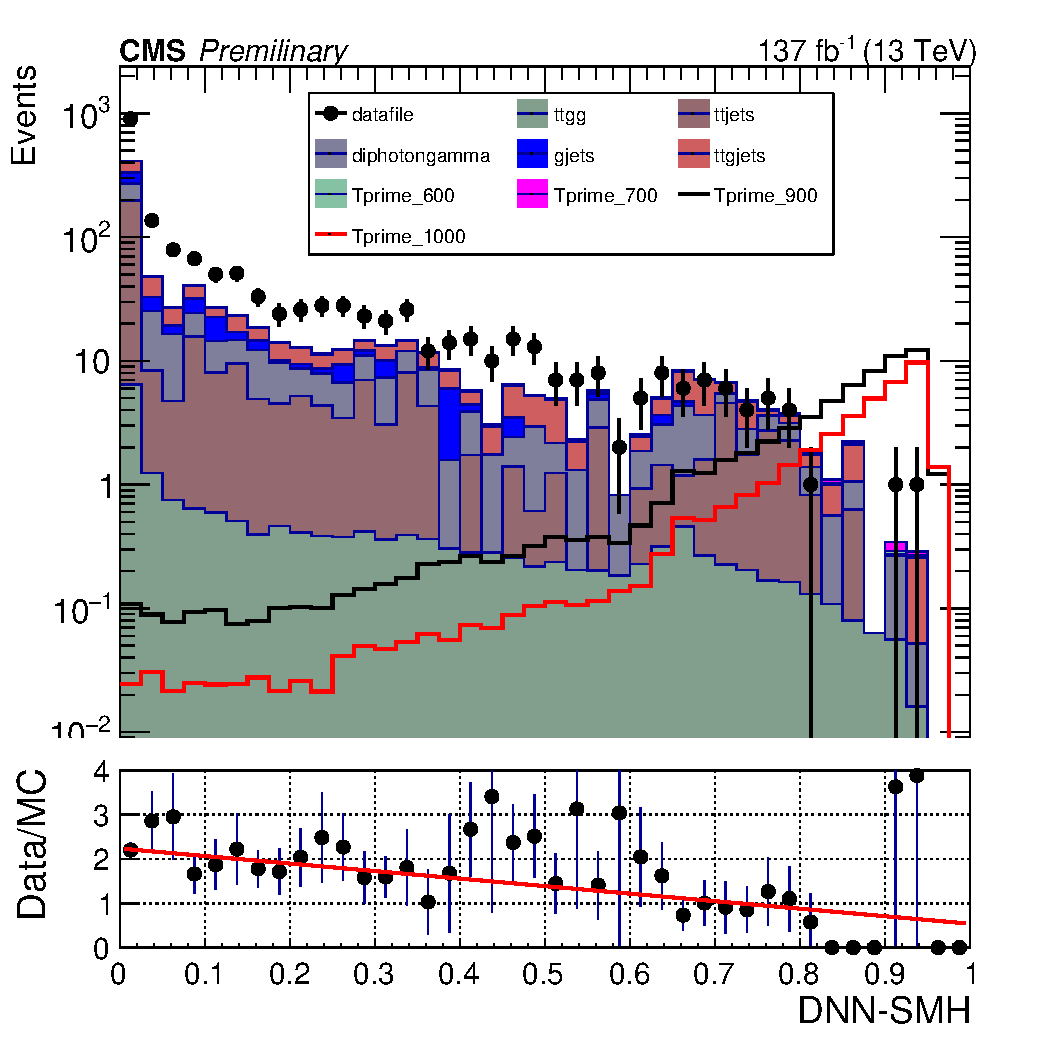
\includegraphics[width=\textwidth]{figure_4/Stacked_plot_DNN_800-1000_with_diphoton_cuts.pdf}
        %  \caption{$y=3sinx$}
        %  \label{fig:three sin x}
     \end{subfigure}
     \hfill
     \begin{subfigure}[b]{0.3\textwidth}
         \centering
         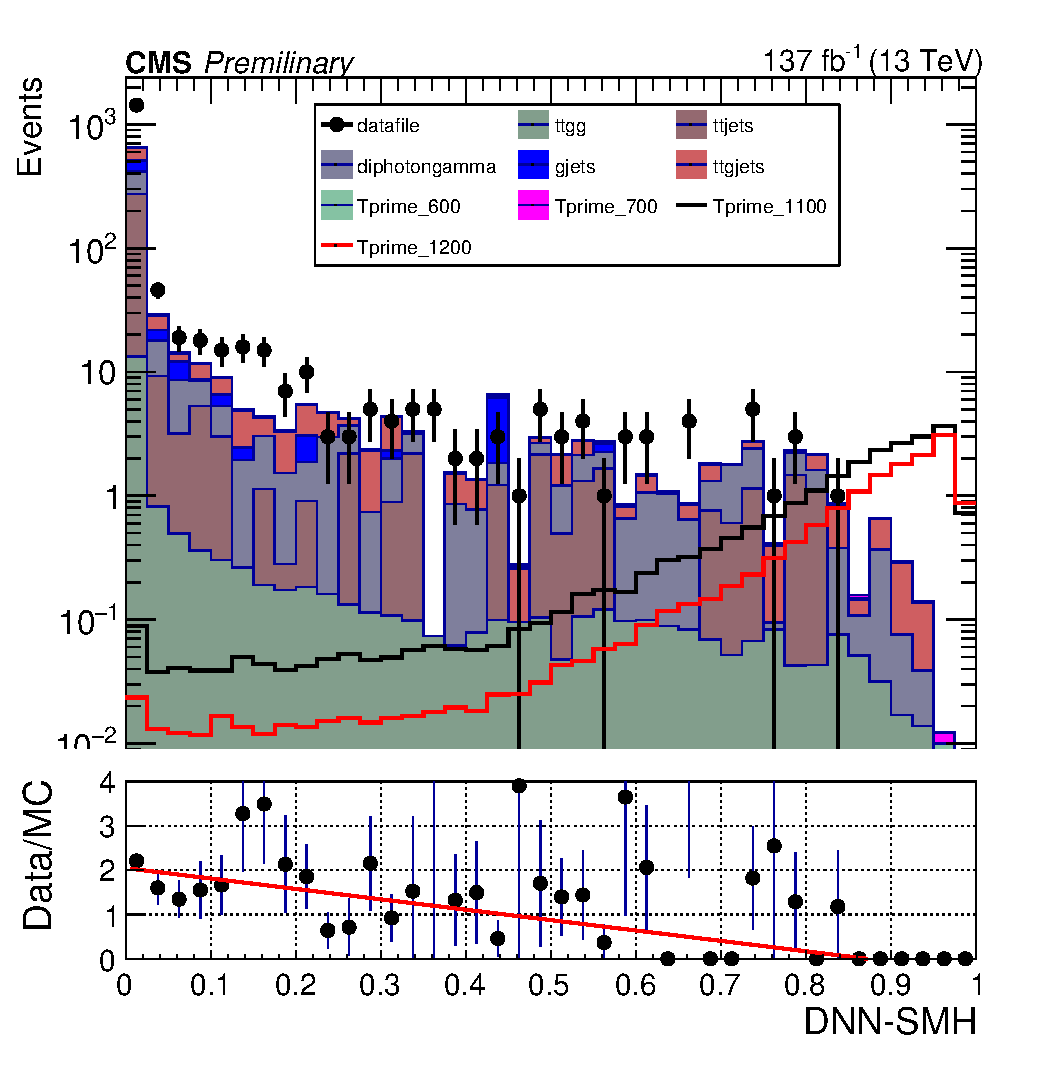
\includegraphics[width=\textwidth]{figure_4/Stacked_plot_DNN_1100-1200_with_diphoton_cuts.pdf}
        %  \caption{$y=3sinx$}
        %  \label{fig:three sin x}
     \end{subfigure}
    \label{fig:stacked_plot_DNN_100}
    \caption{The stacked ratio plot corresponding to the output after testing of different backgrounds, and signal over the DNN score.}
\end{figure}

With the help of linear fit $Y = mx+c$, the ratio plot of the data and the Monte Carlo were fitted and corresponding output of the slope and intercept, as given in \autoref{tab:my_label_DNN_1} were used to scale the values and again the stacked ratio plot were plotted as shown in the \autoref{fig:stacked_scaled_plot_DNN_200}. 


\begin{table}[H]
    \centering
    \begin{tabular}{|c|c|c|}\hline
     Model (DNN)   & Slope & Intercept \\ \hline
      TPrime[600-700]   &  -1.52828 $\pm$ 0.342382 & 2.21165 $\pm$ 0.155941  \\
       TPrime[800-1000]   &  -1.6964 $\pm$ 0.34357 & 2.2345 $\pm$ 0.139593 \\
          TPrime[1100-1200]   &  -2.34415 $\pm$ 0.477097 &  2.04436 $\pm$  0.122349  \\\hline
    \end{tabular}
    \caption{Slope and intercept after linear fitting in the DNN}
    \label{tab:my_label_DNN_1}
\end{table}




\begin{table}[H]
    \centering
    \begin{tabular}{|c|c|c|}\hline
     Model (BDT)   & Slope & Intercept \\ \hline
      TPrime[600-700]   &  -2.55526 $\pm$ 0.406623 & 2.58306 $\pm$ 0.181075  \\
       TPrime[800-1000]   &  -2.95575 $\pm$ 0.537814 & 2.50859 $\pm$ 0.182962 \\
          TPrime[1100-1200]   &  -3.16991 $\pm$ 0.483748 &  2.38726 $\pm$  0.153541  \\\hline
    \end{tabular}
    \caption{Slope and intercept after linear fitting in the BDT}
    \label{tab:my_label_BDT_table}
\end{table}



\begin{figure}[H]
     \centering
     \begin{subfigure}[b]{0.3\textwidth}
         \centering
         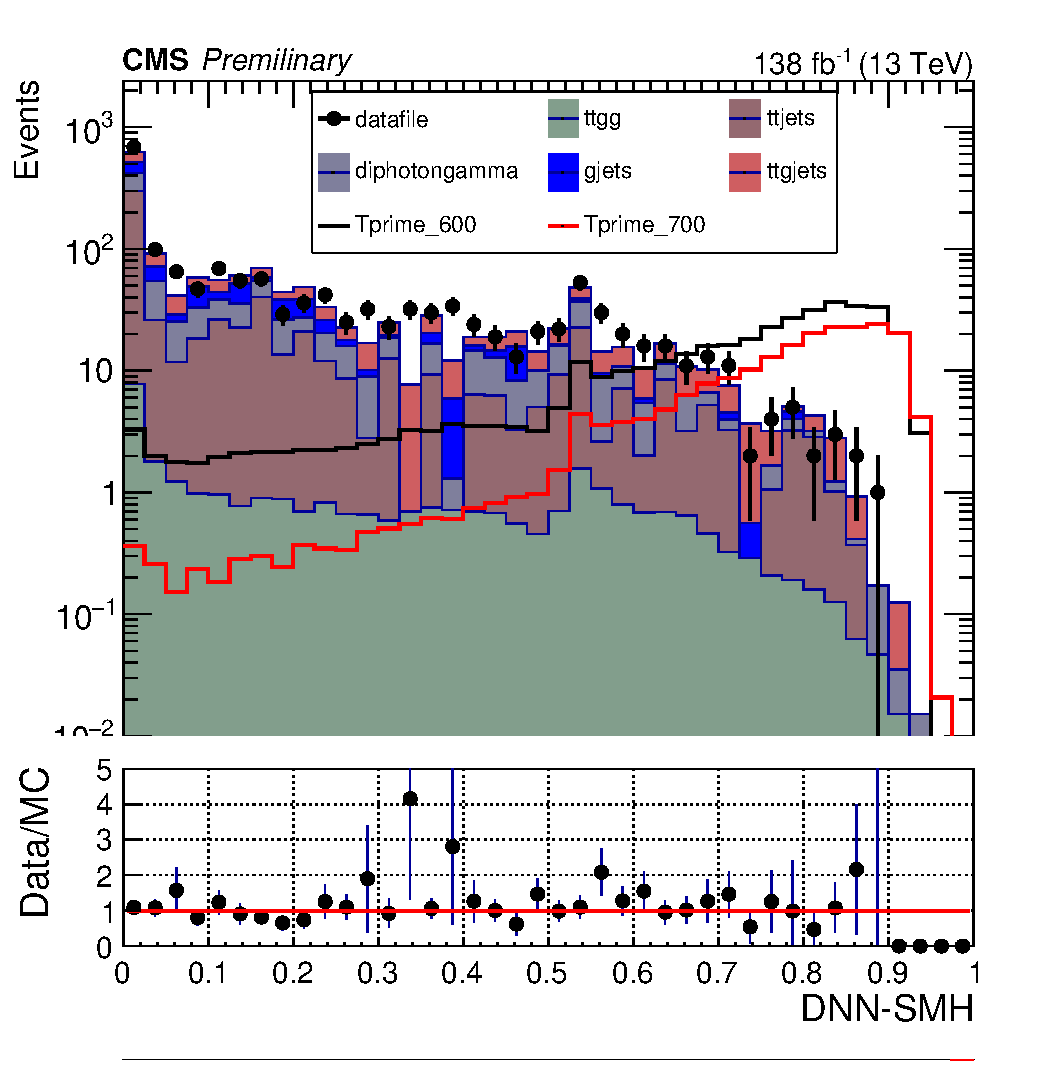
\includegraphics[width=\textwidth]{figure_4/Stacked_plot_DNN_600-700_with_diphoton_cuts_Scaled_inputs.pdf}
        %  \caption{$y=x$}
         \label{fig:y equals x}
     \end{subfigure}
     \hfill
     \begin{subfigure}[b]{0.3\textwidth}
         \centering
         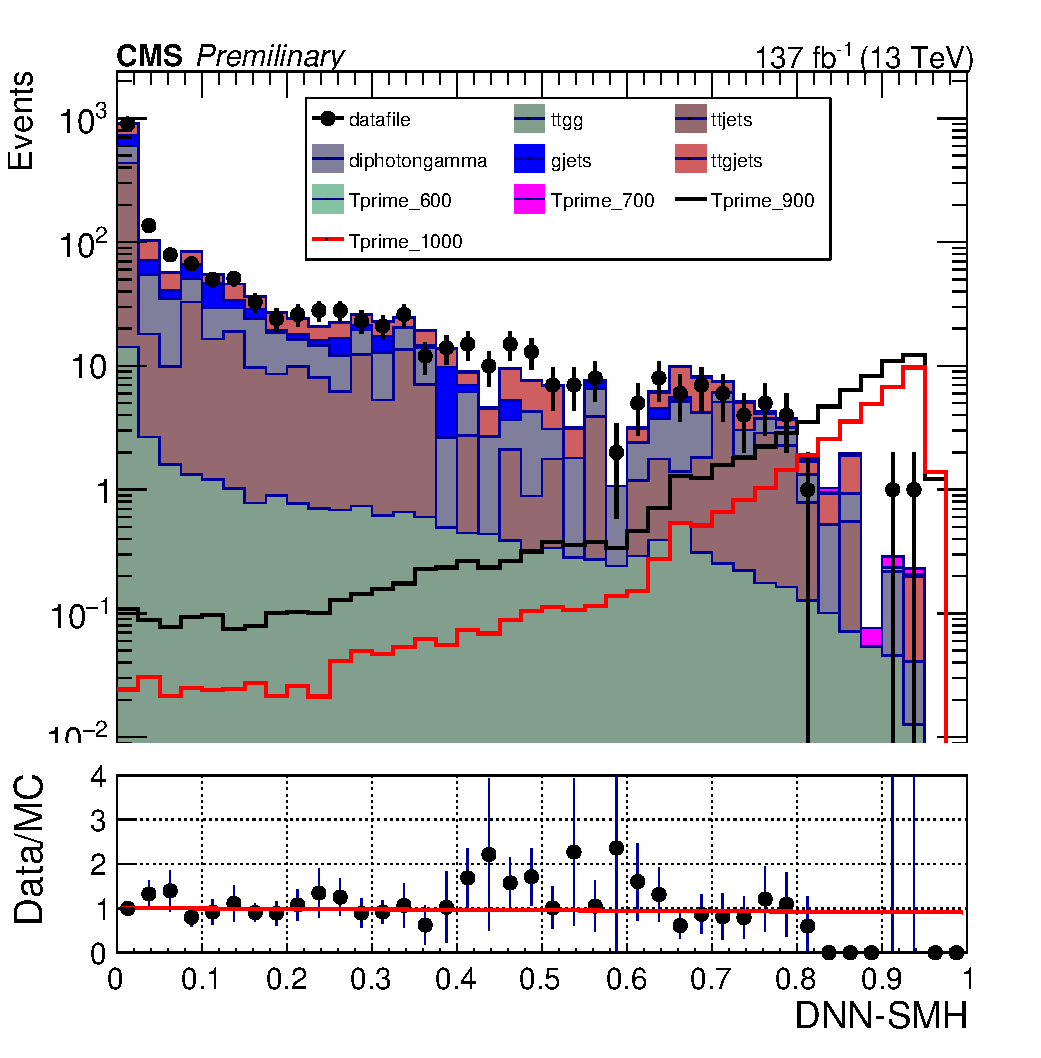
\includegraphics[width=\textwidth]{figure_4/Stacked_plot_DNN_800-1000_with_diphoton_cuts_scaled_inputs.pdf}
        %  \caption{$y=3sinx$}
         \label{fig:three sin x}
     \end{subfigure}
    \hfill
     \begin{subfigure}[b]{0.3\textwidth}
         \centering
         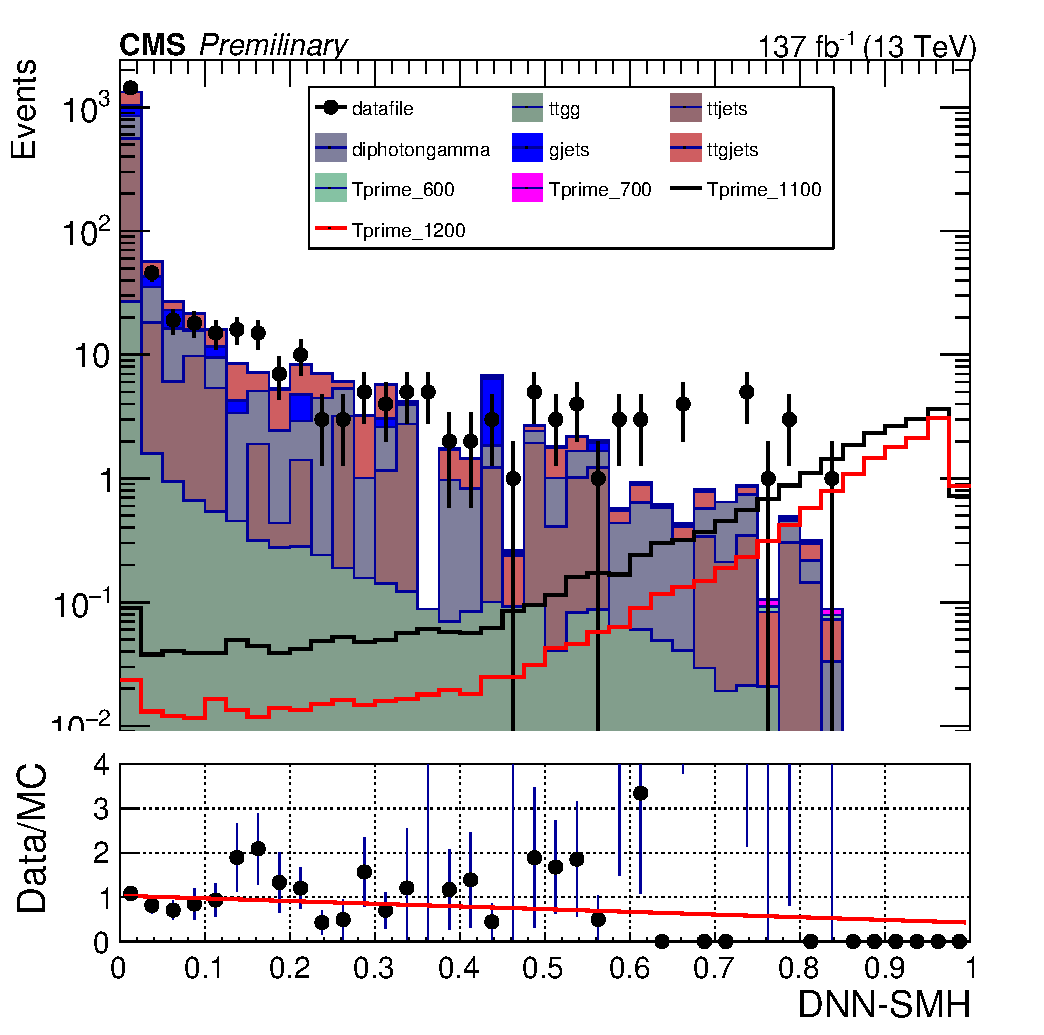
\includegraphics[width=\textwidth]{figure_4/Stacked_plot_DNN_1100-1200_with_diphoton_cuts_scaled_inputs.pdf}
        %  \caption{$y=3sinx$}
         \label{fig:three sin x}
     \end{subfigure}
     \label{fig:stacked_scaled_plot_DNN_200}
     \caption{The stacked ratio plot corresponding to the output after testing of different backgrounds, and signal over the DNN score after linear fitting the ratio plot and scaled the input. Here, the data are matching with the monte carlo.}
\end{figure}



As in the DNN the process, after testing on the DNN score the coutput were plotted as the stacked ratio plot, the corresponding plot to the training with Boosted Decision Tree(BDT) can be seen in the \autoref{fig:BDT_output_11}. 


\begin{figure}[H]
     \centering
     \begin{subfigure}[b]{0.3\textwidth}
         \centering
         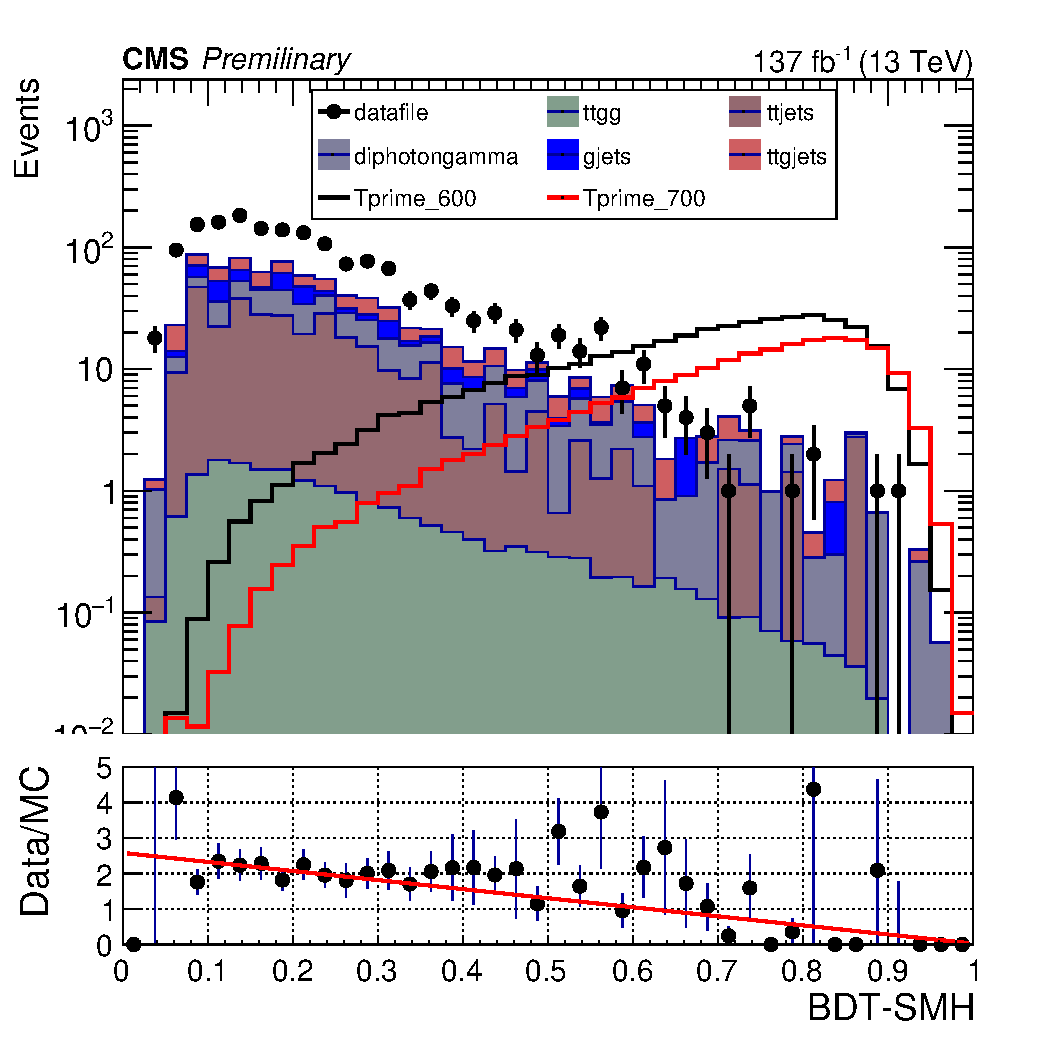
\includegraphics[width=\textwidth]{BDT_Output/Stacked_plot_BDT_600-700_with_diphoton_cuts_inputs.pdf}
        %  \caption{$y=x$}
         \label{fig:y equals x}
     \end{subfigure}
     \hfill
     \begin{subfigure}[b]{0.3\textwidth}
         \centering
         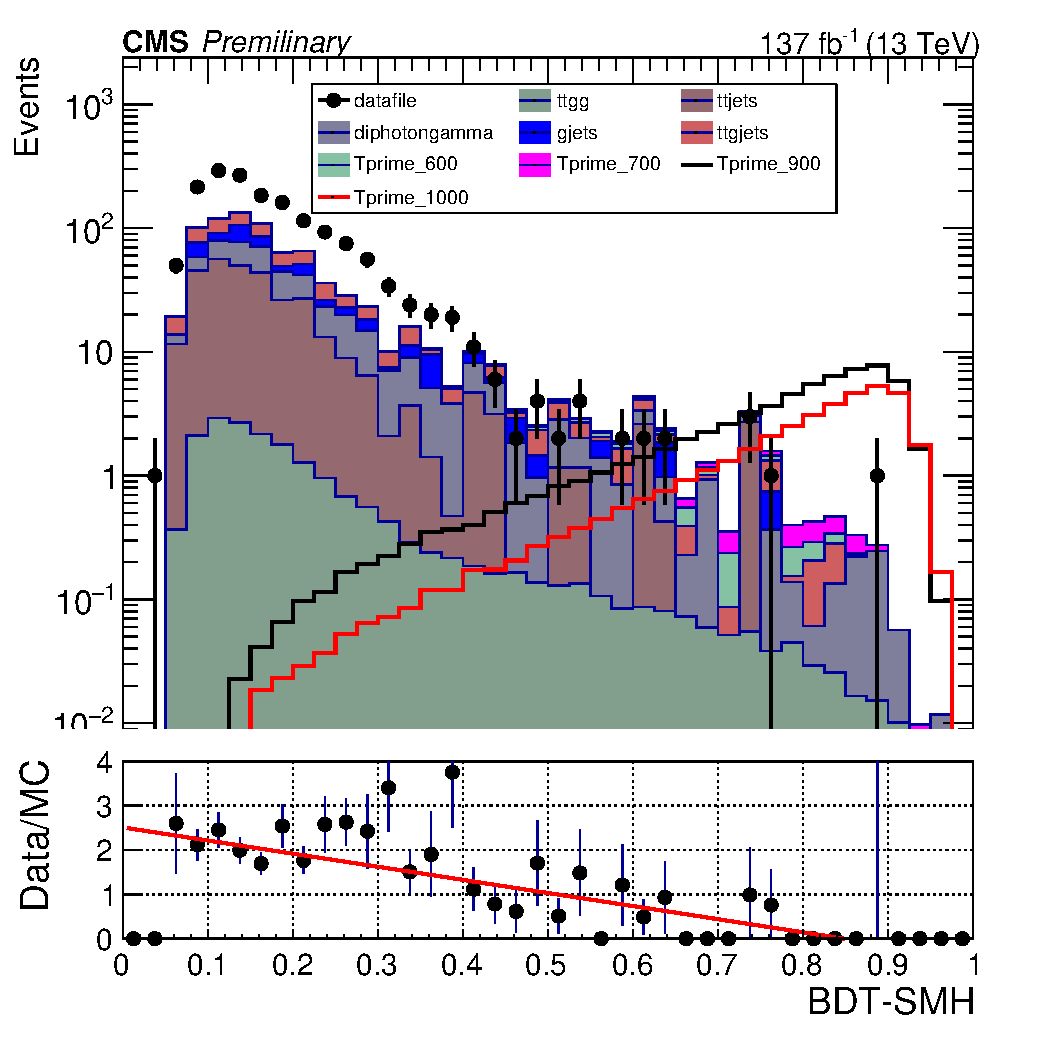
\includegraphics[width=\textwidth]{BDT_Output/Stacked_plot_BDT_800-1000_with_diphoton_cuts_inputs.pdf}
         
        %  \caption{$y=3sinx$}
         \label{fig:three sin x}
     \end{subfigure}
     \hfill
     \begin{subfigure}[b]{0.3\textwidth}
         \centering
         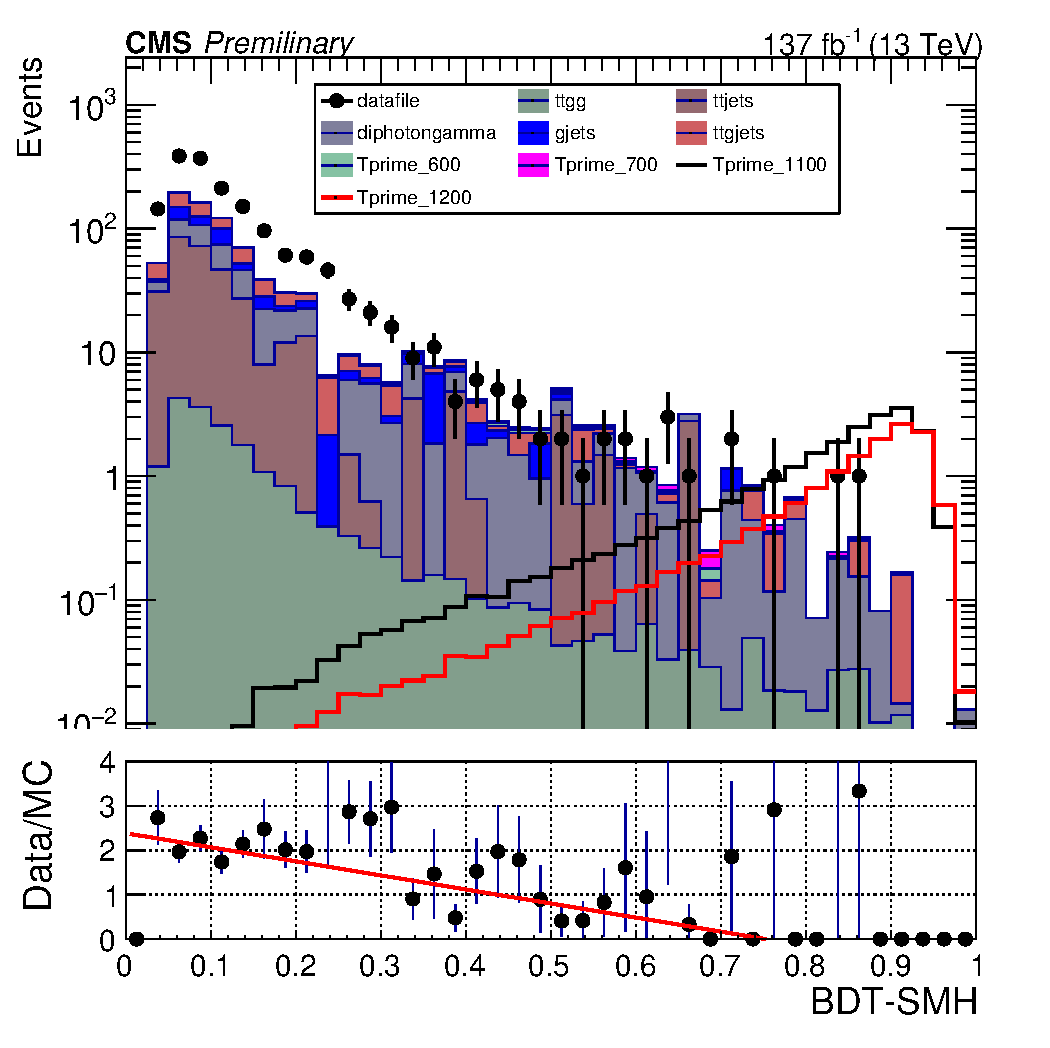
\includegraphics[width=\textwidth]{BDT_Output/Stacked_plot_BDT_1100-1200_with_diphoton_cuts_inputs.pdf}
        %  \caption{$y=3sinx$}
         \label{fig:three sin x}
     \end{subfigure}
     \label{fig:BDT_output_11}
     \caption{The stacked ratio plot corresponding to the output after testing of different backgrounds, and signal over the DNN score.}
\end{figure}


The Stacked ration plot of BDT output after linear fit and scaling with the corresponding parameters is in \autoref{fig:BDT_ouput_Fitted}.



% \section{Di-photon cuts with scaled inputs(BDT)}
\begin{figure}[H]
     \centering
     \begin{subfigure}[b]{0.3\textwidth}
         \centering
         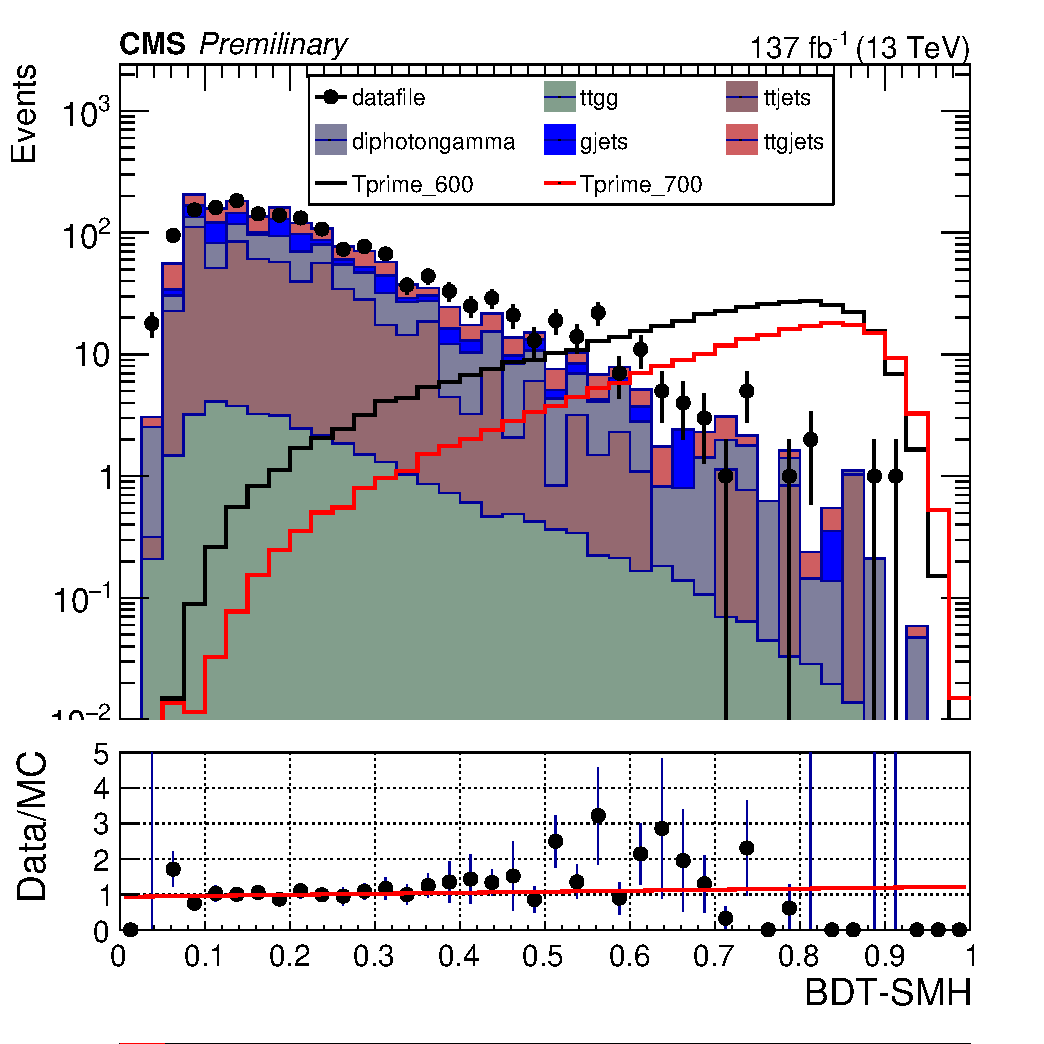
\includegraphics[width=\textwidth]{BDT_Output/Stacked_plot_BDT_600-700_with_diphoton_cuts_with_scaled_inputs.pdf}
        %  \caption{$y=x$}
         \label{fig:y equals x}
     \end{subfigure}
     \hfill
     \begin{subfigure}[b]{0.3\textwidth}
         \centering
         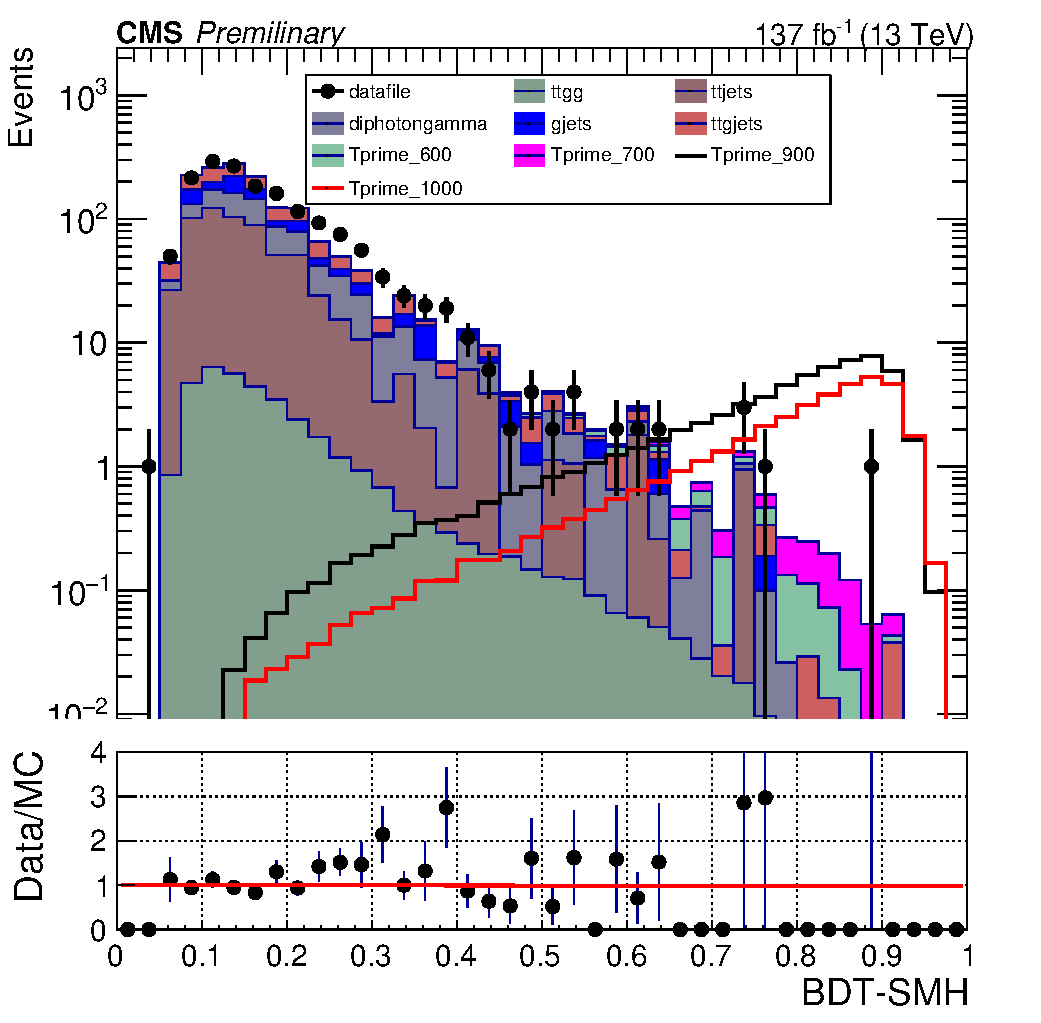
\includegraphics[width=\textwidth]{BDT_Output/Stacked_plot_BDT_800-1000_with_diphoton_cuts_with_Scaled_inputs.pdf}
        %  \caption{$y=3sin/x$}
         \label{fig:three sin x}
     \end{subfigure}
    \hfill
     \begin{subfigure}[b]{0.3\textwidth}
         \centering
         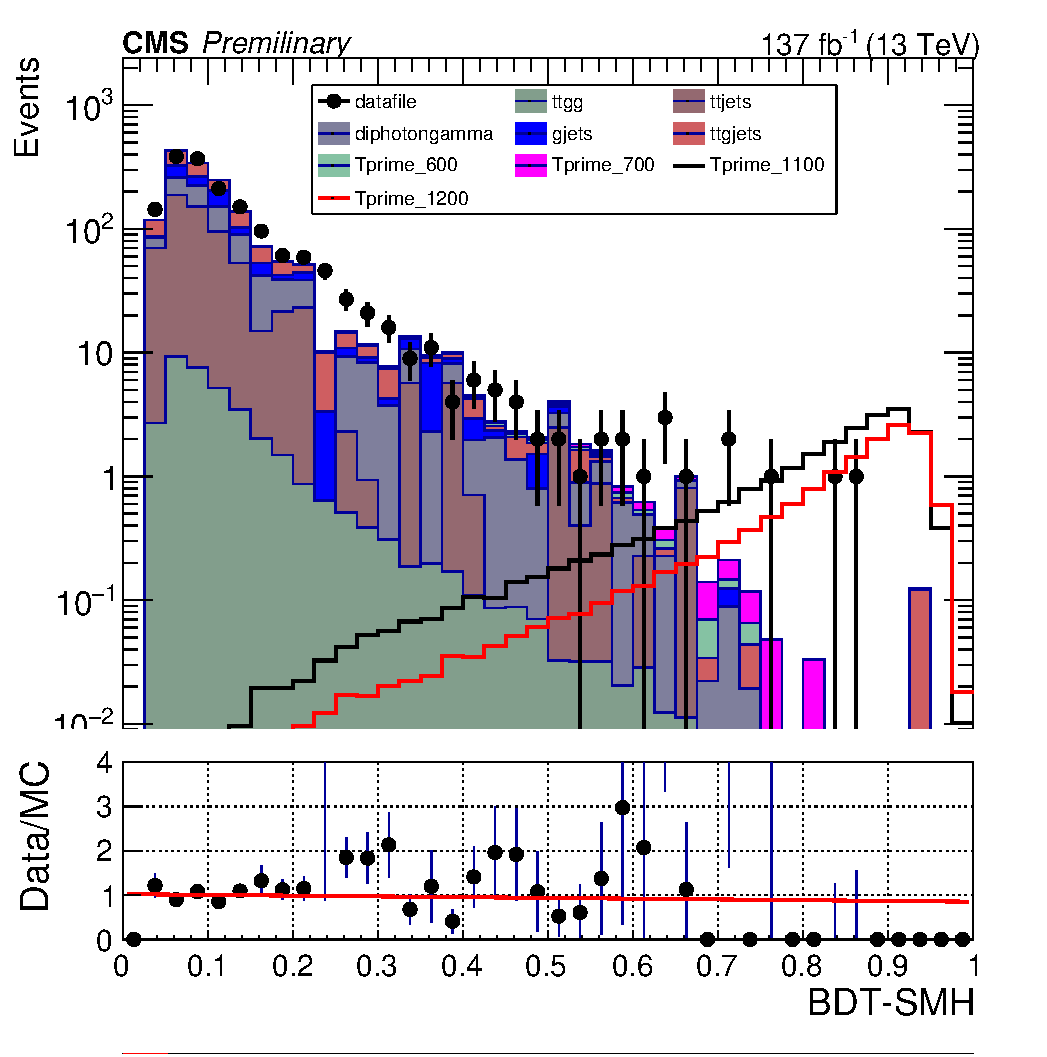
\includegraphics[width=\textwidth]{BDT_Output/Stacked_plot_BDT_1100-1200_with_diphoton_cuts_with_scaled_inputs.pdf}
        %  \caption{$y=3sinx$}
         \label{fig:three sin x}
     \end{subfigure}
     \label{fig:BDT_ouput_Fitted}
     \caption{The stacked ratio plot corresponding to the output after testing of different backgrounds, and signal over the BDT score after linear fitting the ratio plot and scaled the input. Here, the data are matching with the monte carlo .}
\end{figure}


%%%%%%%%%%%%%%%%%%%%%%%%%%%%%%%%%%%%%%%%%%%%%%%%%%%%%%%%%%%%5
%%%%%%%%%%%%%%%%%%%%%%%%%%%%%%%%%%%%%%%%%%%%%%%%%%%%%%%%%%%%5
%%%%%%%%%%%%%%%%%%%%%%%%%%%%%%%%%%%%%%%%%%%%%%%%%%%%%%%%%%%%5
%%%%%%%%%%%%%%%%%%%%%%%%%%%%%%%%%%%%%%%%%%%%%%%%%%%%%%%%%%%%5
%%%%%%%%%%%%%%%%%%%%%%%%%%%%%%%%%%%%%%%%%%%%%%%%%%%%%%%%%%%%5
%%%%%%%%%%%%%%%%%%%%%%%%%%%%%%%%%%%%%%%%%%%%%%%%%%%%%%%%%%%%5
%%%%%%%%%%%%%%%%%%%%%%%%%%%%%%%%%%%%%%%%%%%%%%%%%%%%%%%%%%%%5


\section{BDT and DNN Comparisons}
The different machine learning techniques comparisons can be seen in the following figures.

\begin{figure}[H]
     \centering
     \begin{subfigure}[b]{0.45\textwidth}
         \centering
         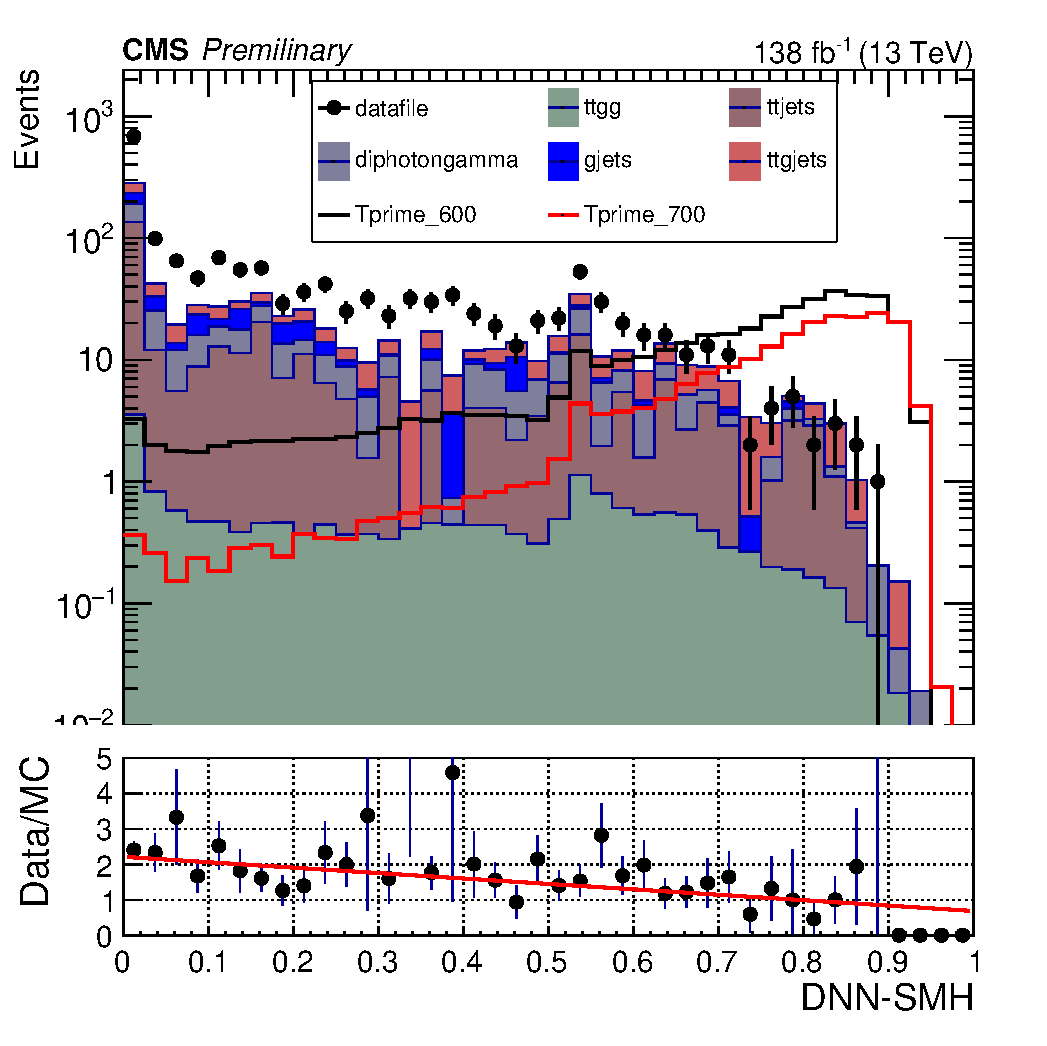
\includegraphics[width=\textwidth]{figure_4/Stacked_plot_DNN_600-700_with_diphoton_cuts.pdf}
        %  \caption{$y=x$}
         \label{fig:y equals x}
     \end{subfigure}
     \hfill
     \begin{subfigure}[b]{0.45\textwidth}
         \centering
         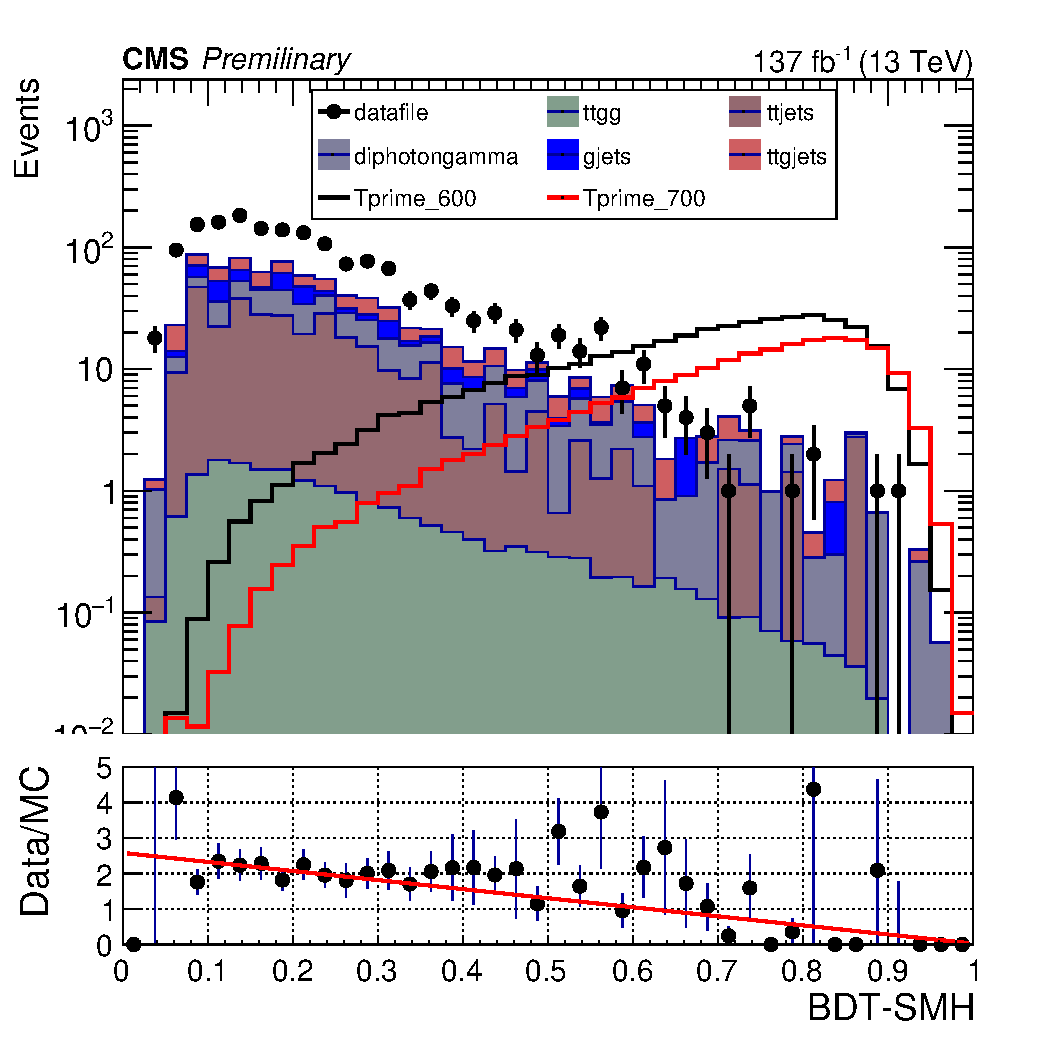
\includegraphics[width=\textwidth ]{BDT_Output/Stacked_plot_BDT_600-700_with_diphoton_cuts_inputs.pdf}
        %  \caption{$y=3sinx$}
         \label{fig:three sin x}
     \end{subfigure}
     \label{fig:Comaprision_1}
     \caption{Comparison for the BDT and DNN output corresponding to the training for Tprime[600-700GeV] and testing on NRB, SMH, and Tprime at 600GeV and 700GeV as given in \autoref{tab:my_label_DNN_1} and \autoref{tab:my_label_BDT_table}.}
\end{figure}




\begin{figure}[H]
     \centering
     \begin{subfigure}[b]{0.47\textwidth}
         \centering
         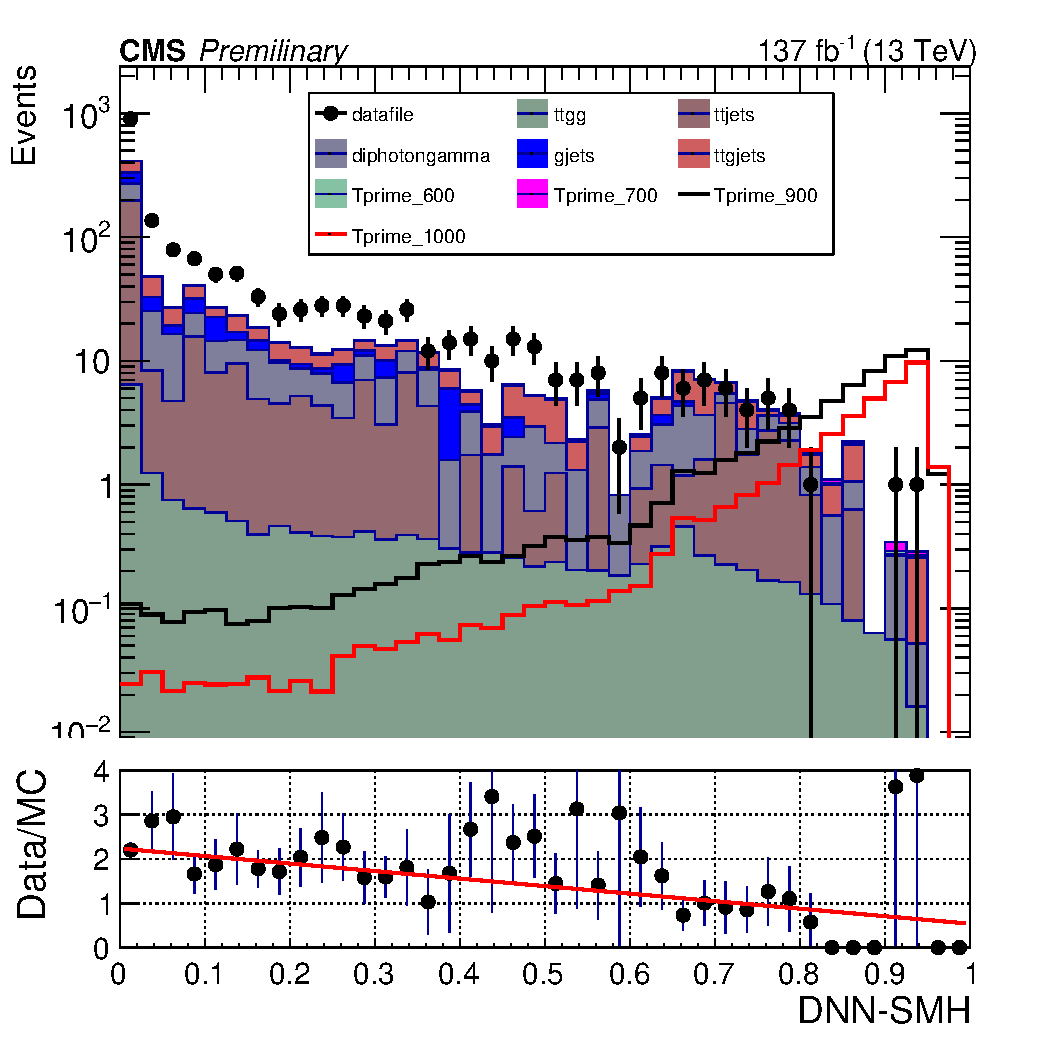
\includegraphics[width=\textwidth]{figure_4/Stacked_plot_DNN_800-1000_with_diphoton_cuts.pdf}
        %  \caption{$y=x$}
         \label{fig:y equals x}
     \end{subfigure}
     \hfill
     \begin{subfigure}[b]{0.47\textwidth}
         \centering
         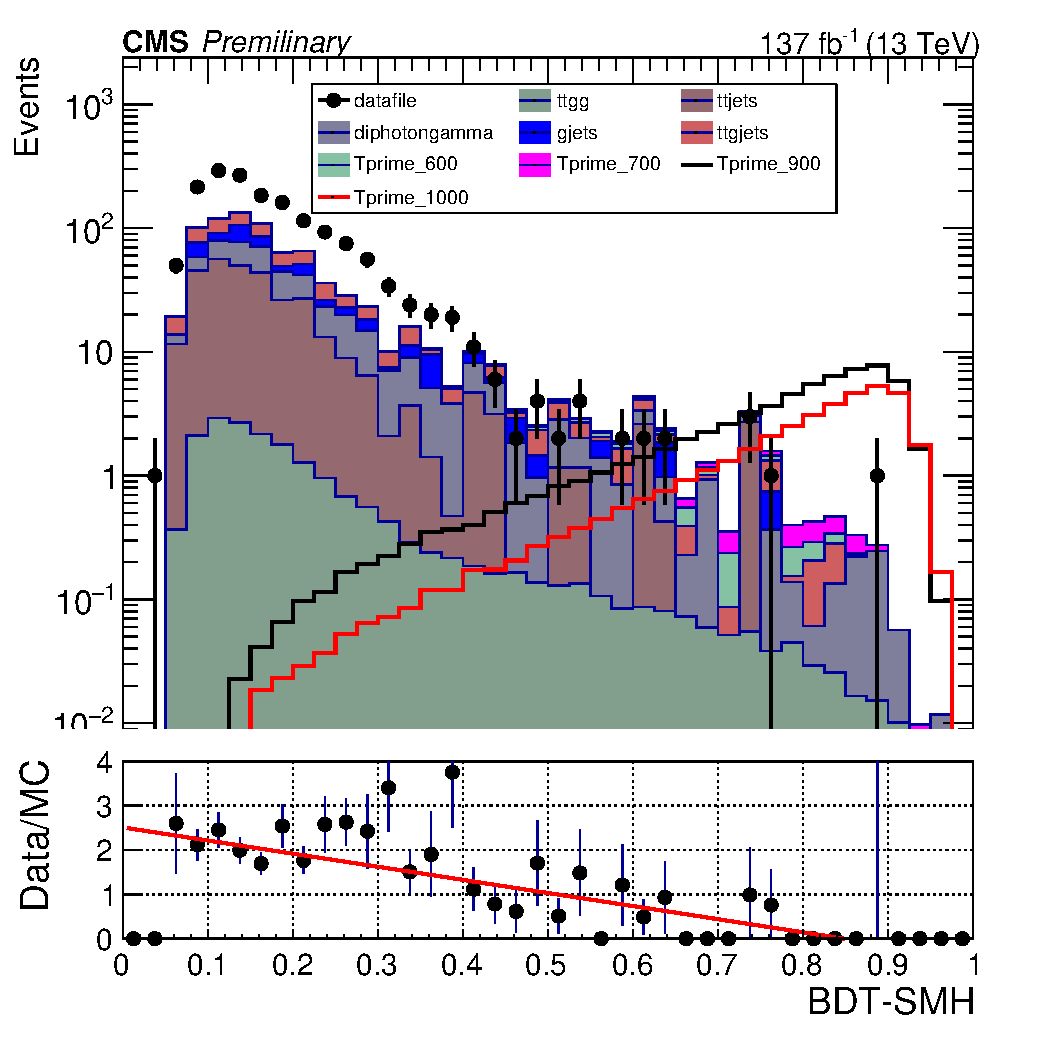
\includegraphics[width=\textwidth]{BDT_Output/Stacked_plot_BDT_800-1000_with_diphoton_cuts_inputs.pdf}
        %  \caption{$y=3sinx$}
         \label{fig:three sin x}
     \end{subfigure}
     \label{fig:Comaprision_2}
     \caption{Comparison for the BDT and DNN output corresponding to the training for Tprime[800-1000GeV] and testing on NRB, SMH, and Tprime at 600GeV, 700GeV, 900GeV, and 1000GeV as given in \autoref{tab:my_label_DNN_1} and \autoref{tab:my_label_BDT_table}.}
\end{figure}




\begin{figure}[H]
     \centering
     \begin{subfigure}[b]{0.47\textwidth}
         \centering
         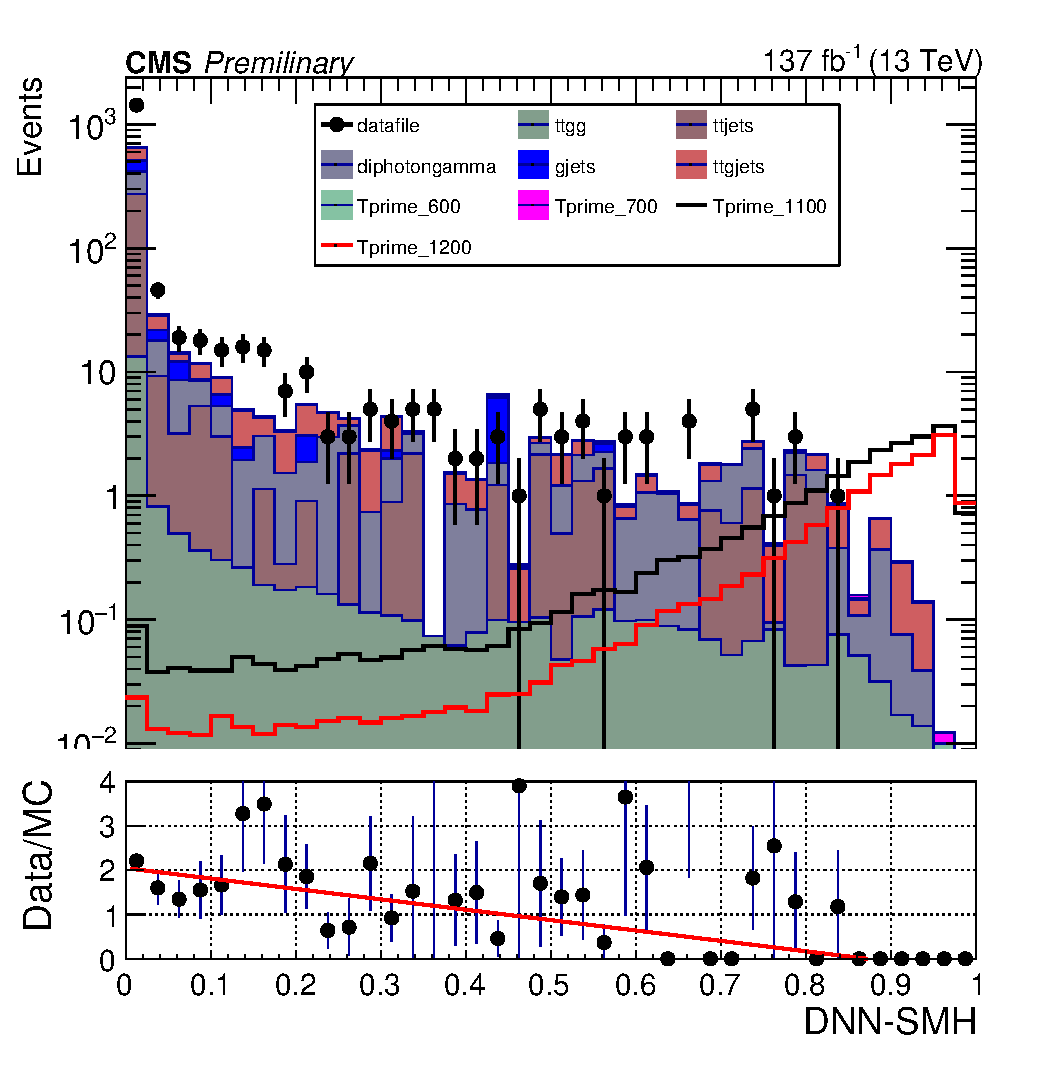
\includegraphics[width=\textwidth]{figure_4/Stacked_plot_DNN_1100-1200_with_diphoton_cuts.pdf}
        %  \caption{$y=x$}
         \label{fig:y equals x}
     \end{subfigure}
     \hfill
     \begin{subfigure}[b]{0.47\textwidth}
         \centering
         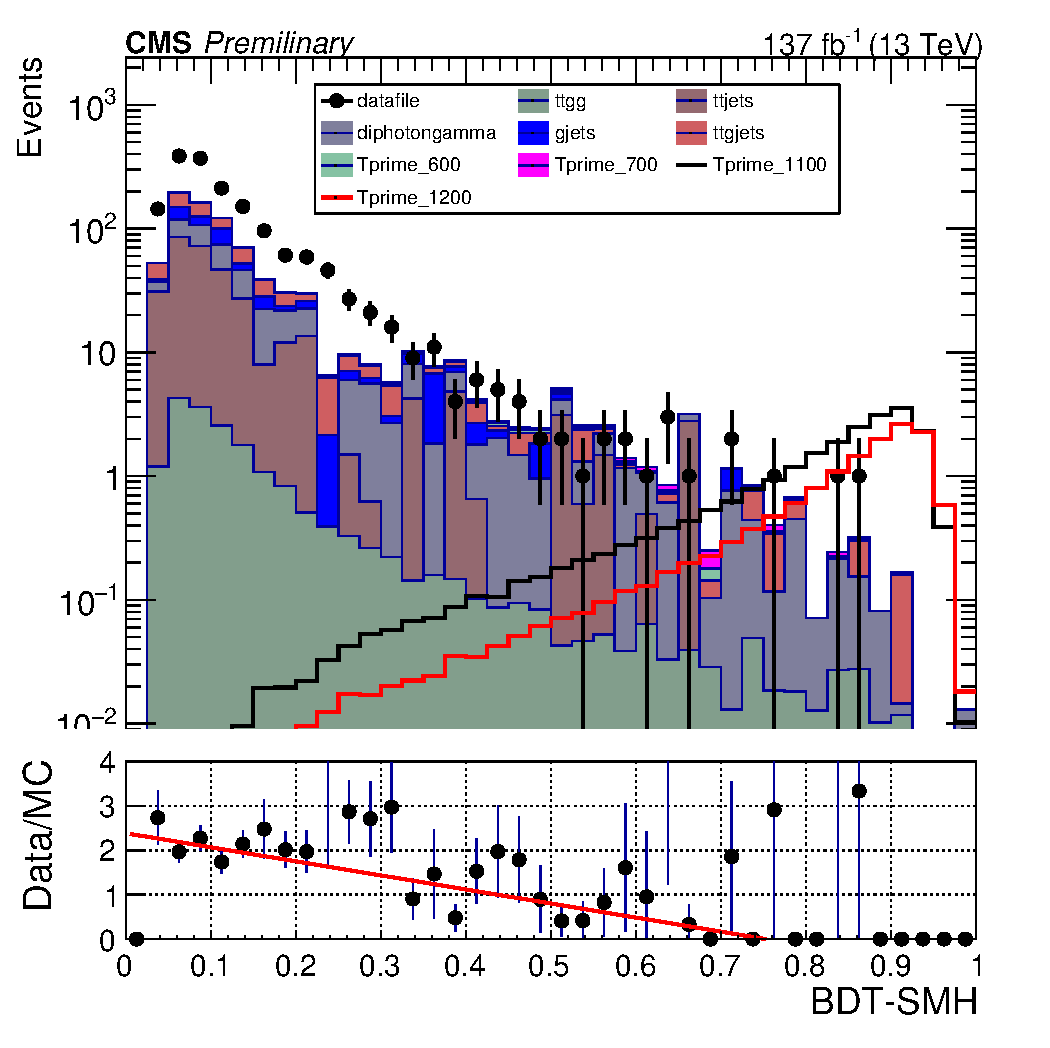
\includegraphics[width=\textwidth]{BDT_Output/Stacked_plot_BDT_1100-1200_with_diphoton_cuts_inputs.pdf}
        %  \caption{$y=3sinx$}
         \label{fig:three sin x}
     \end{subfigure}
    \hfill
     \label{fig:Comaprision_3}
     \caption{Comparison for the BDT and DNN output corresponding to the training for Tprime[1100-1200GeV] and testing on NRB, SMH, and Tprime at 600GeV, 700GeV, 1100GeV, and 1200GeV as given in \autoref{tab:my_label_DNN_1} and \autoref{tab:my_label_BDT_table}.}
\end{figure}

%%%%%%%%%%%%%%%%Scaled Inputs%%%%%%%%%%%%%%%%%%%%


\begin{figure}[H]
     \centering
     \begin{subfigure}[b]{0.47\textwidth}
         \centering
         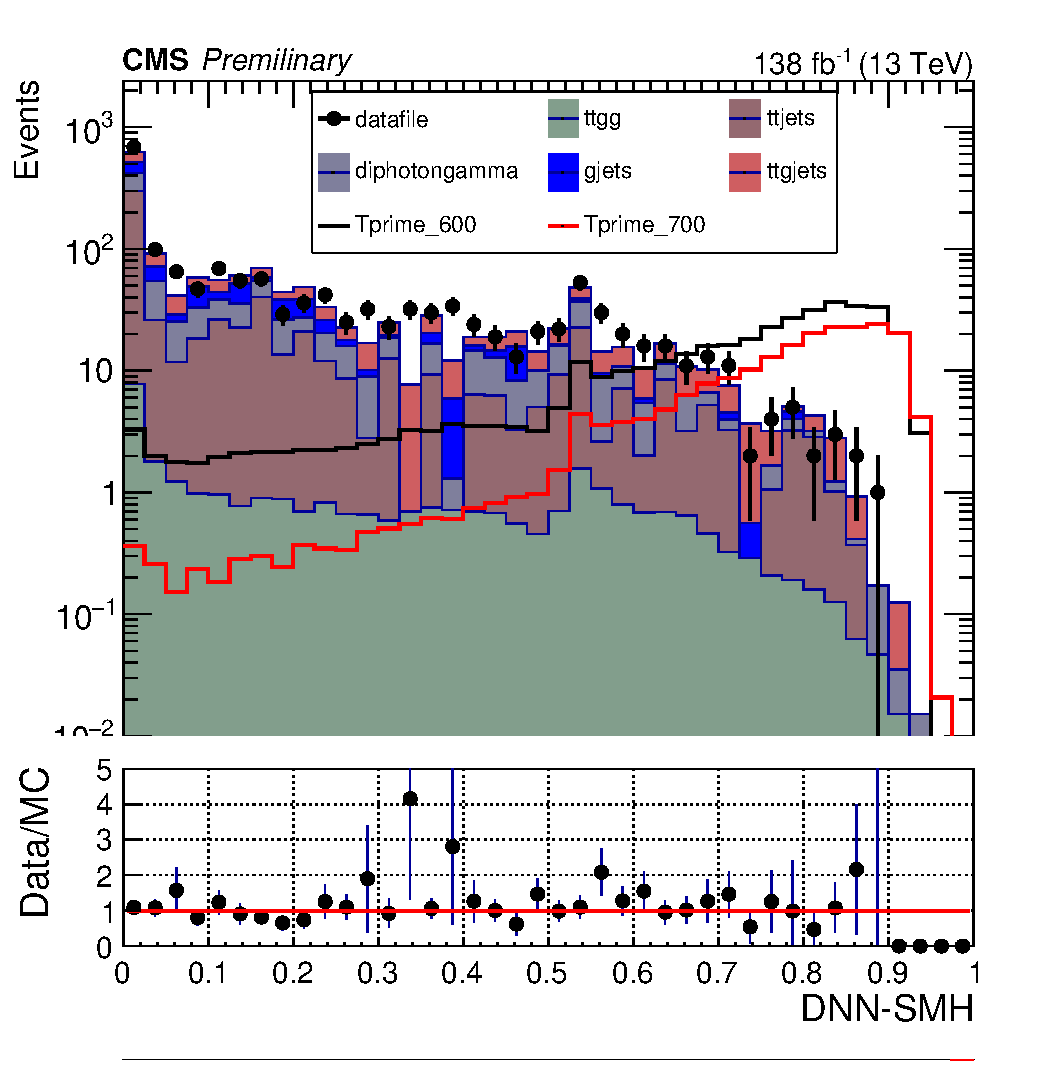
\includegraphics[width=\textwidth]{figure_4/Stacked_plot_DNN_600-700_with_diphoton_cuts_Scaled_inputs.pdf}
        %  \caption{$y=x$}
         \label{fig:y equals x}
     \end{subfigure}
     \hfill
     \begin{subfigure}[b]{0.47\textwidth}
         \centering
         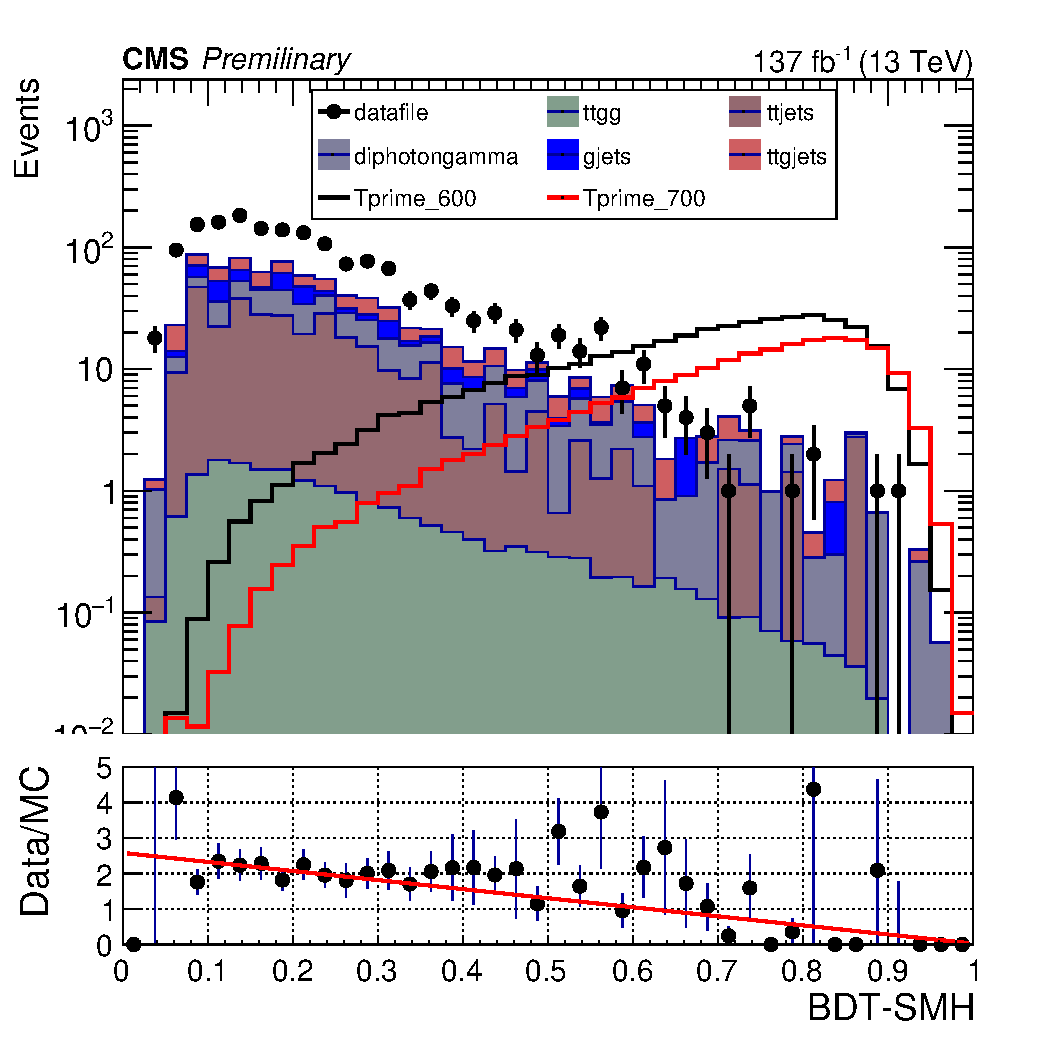
\includegraphics[width=\textwidth]{BDT_Output/Stacked_plot_BDT_600-700_with_diphoton_cuts_inputs.pdf}
        %  \caption{$y=3sinx$}
         \label{fig:three sin x}
     \end{subfigure}
    \hfill
     \label{fig:Comaprision_4}
     \caption{Comparision for the BDT and DNN output corresponding to the training for Tprime[600-700GeV] and testing on NRB, SMH, and Tprime at 600GeV and 700GeV with the scaled inputs after fitted parameter of slope and intercept as given in \autoref{tab:my_label_DNN_1} and \autoref{tab:my_label_BDT_table}.}
\end{figure}






\begin{figure}[H]
     \centering
     \begin{subfigure}[b]{0.47\textwidth}
         \centering
         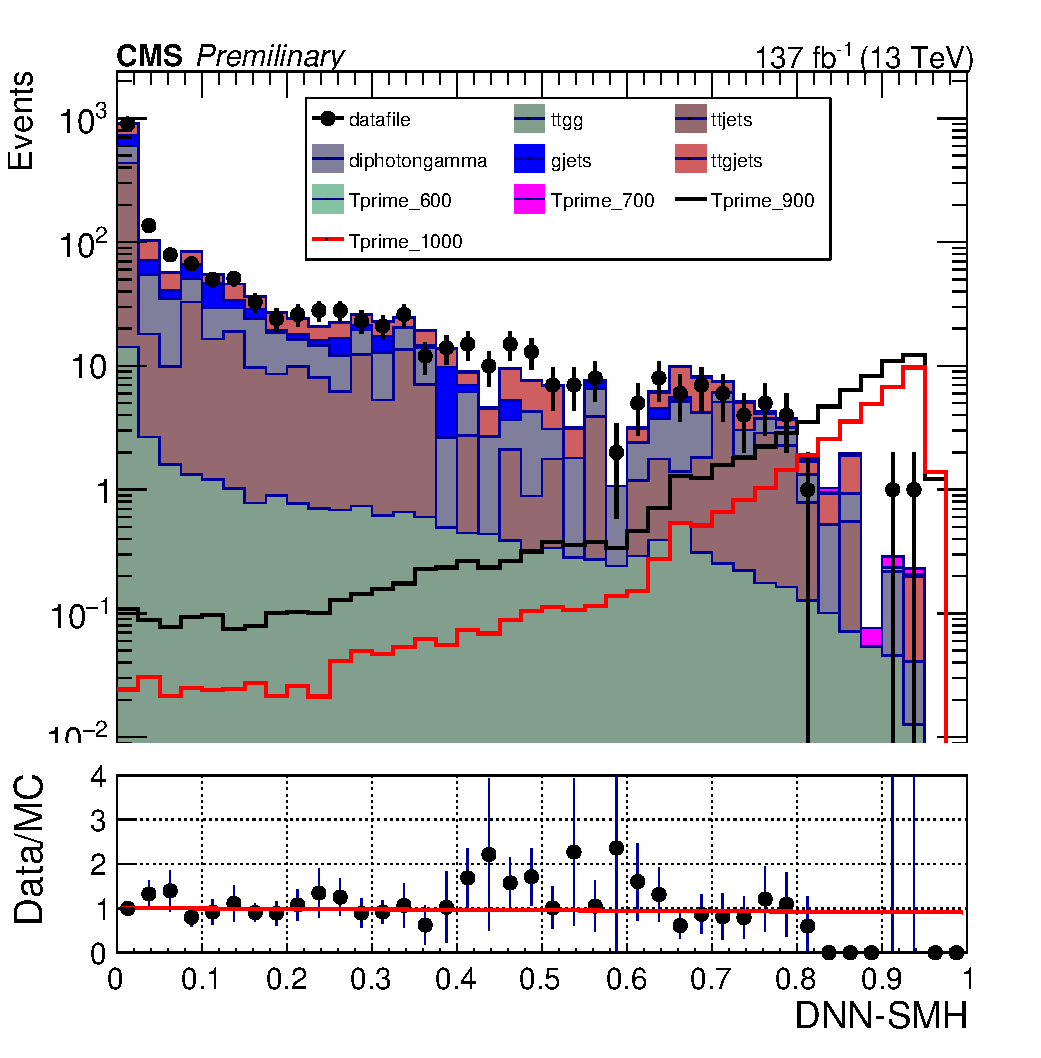
\includegraphics[width=\textwidth]{figure_4/Stacked_plot_DNN_800-1000_with_diphoton_cuts_scaled_inputs.pdf}
        %  \caption{$y=x$}
         \label{fig:y equals x}
     \end{subfigure}
     \hfill
     \begin{subfigure}[b]{0.47\textwidth}
         \centering
         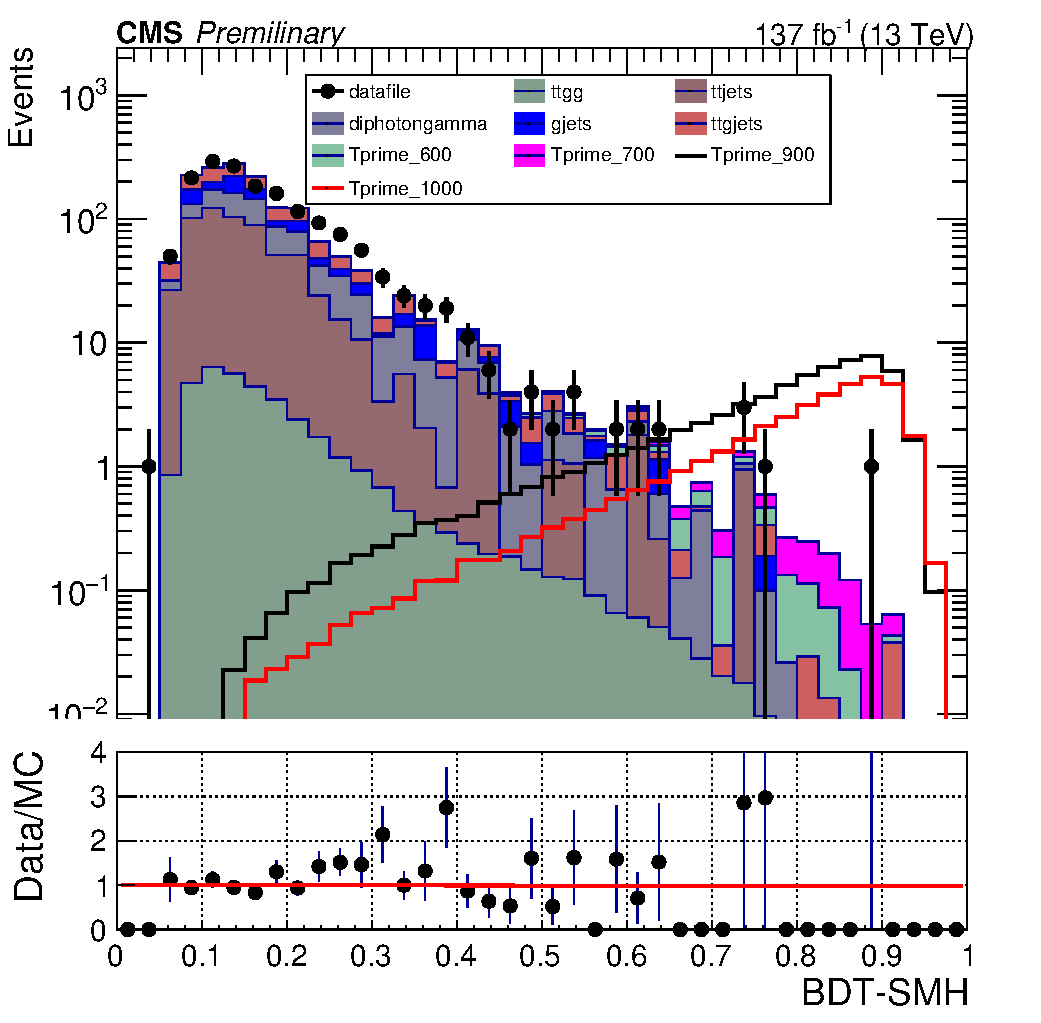
\includegraphics[width=\textwidth]{BDT_Output/Stacked_plot_BDT_800-1000_with_diphoton_cuts_with_Scaled_inputs.pdf}
        %  \caption{$y=3sinx$}
         \label{fig:three sin x}
     \end{subfigure}
    \hfill
     \label{fig:}
     \caption{Comparision for the BDT and DNN output corresponding to the training for Tprime[800-1000GeV] and testing on NRB, SMH, and Tprime at 600GeV, 700GeV, 900GeV, and 1000GeV with the scaled inputs after fitted parameter of slope and intercept as given in \autoref{tab:my_label_DNN_1} and \autoref{tab:my_label_BDT_table}.}
\end{figure}



\begin{figure}[H]
     \centering
     \begin{subfigure}[b]{0.47\textwidth}
         \centering
         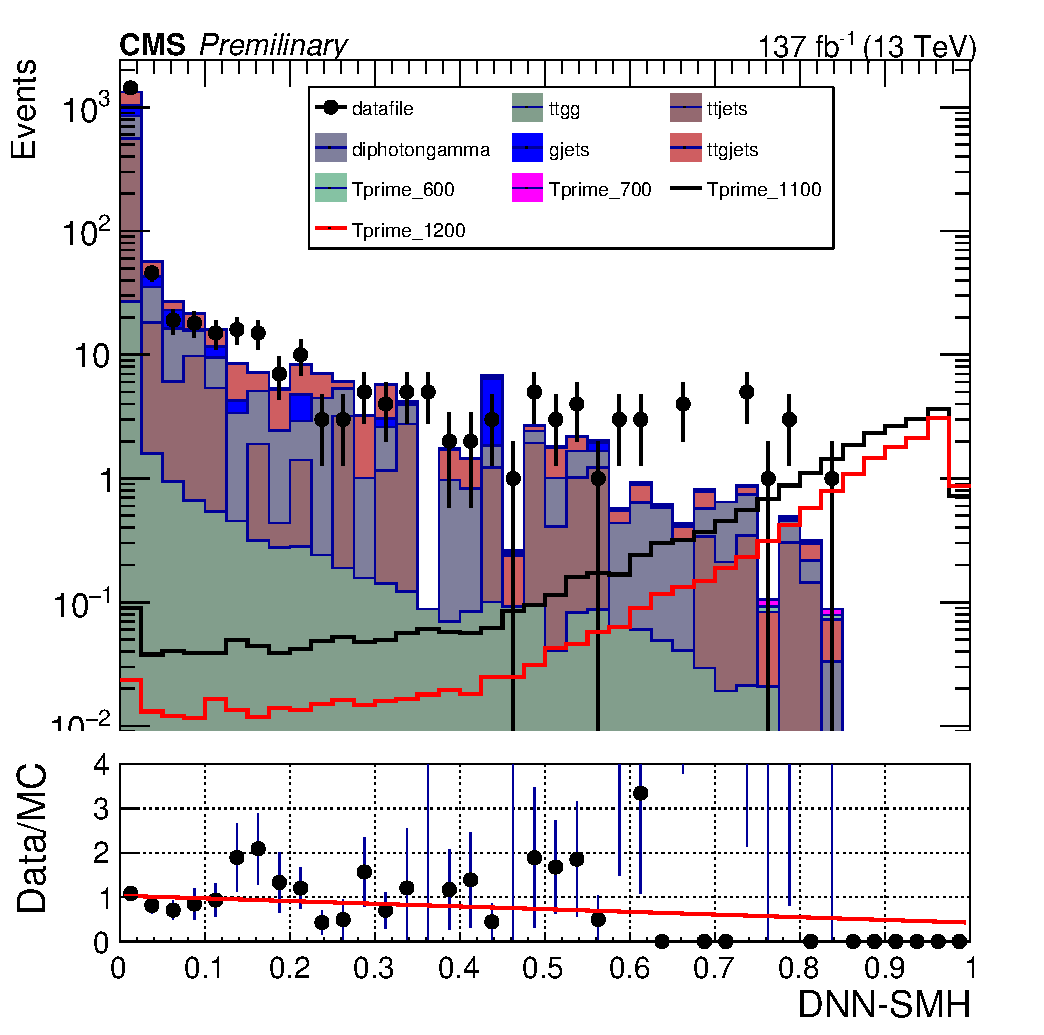
\includegraphics[width=\textwidth]{figure_4/Stacked_plot_DNN_1100-1200_with_diphoton_cuts_scaled_inputs.pdf}
        %  \caption{$y=x$}
         \label{fig:y equals x}
     \end{subfigure}
     \hfill
     \begin{subfigure}[b]{0.47\textwidth}
         \centering
         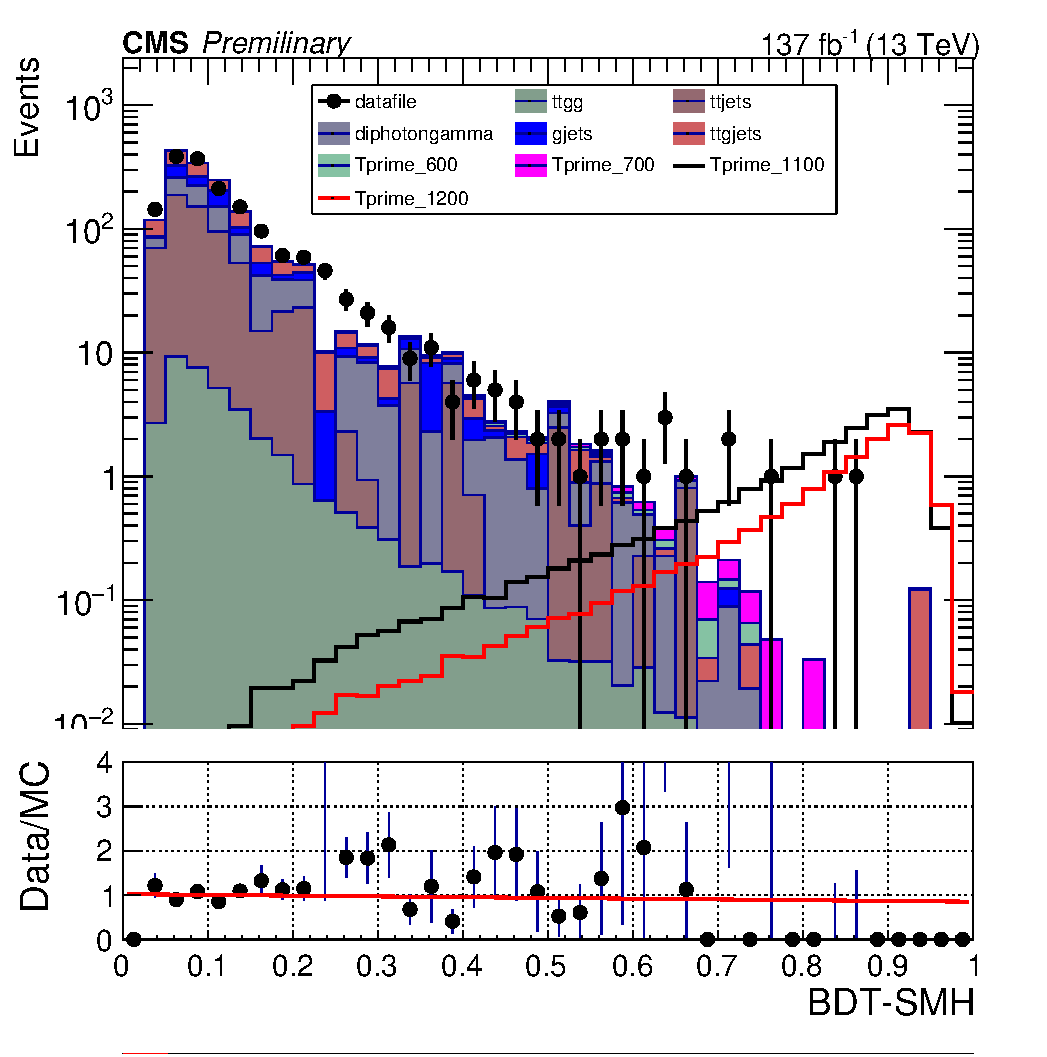
\includegraphics[width=\textwidth]{BDT_Output/Stacked_plot_BDT_1100-1200_with_diphoton_cuts_with_scaled_inputs.pdf}
        %  \caption{$y=3sinx$}
         \label{fig:three sin x}
     \end{subfigure}
    \hfill
     \label{fig:}
     \caption{Comparision for the BDT and DNN output corresponding to the training for Tprime[1100-1200GeV] and testing on NRB, SMH, and Tprime at 600GeV, 700GeV, 1100GeV, and 1200GeV with the scaled inputs after fitted parameter of slope and intercepts as given in \autoref{tab:my_label_DNN_1} and \autoref{tab:my_label_BDT_table}.}
\end{figure}








 \section{Limit Calculation}
Before the use of higgs combine tools on the output variable of the DNN and applying cuts these are the number of the events. This is a frequentist hypothesis to calculate the probability of an hypothesis to be inferred from the data based on a large set of hypothetical experiments, such as the Monte Carlo. 
for the blinded region analysis on 115 < $m_{\gamma\gamma}$ < 135GeV on the monte carlo samples of backgrounds(NRB) have been scaled after the linear fitting of the $\frac{Data}{MC}$ ratio, and scaled to match the data and monte carlo. 
With the cuts applied as in \autoref{tab:my_label_cuts}, the background have been rejected to get most of the signal processes afer testing over the DNN score. 


\begin{table}[H]
    \centering
    \begin{tabular}{c|c} \hline
     Model &  Cuts Applied(position)\\\hline
      ${T'}$[600,700]   &  0.54\\
      $T'$[800,1000]   & 0.76 \\
      $T'$[1100,1200] & 0.80 \\\hline
    \end{tabular}
    \caption{Different cuts applied for different training}
    \label{tab:my_label_cuts}
\end{table}

The inputs sample have been scaled after linear fitting of the ratio plot or applied cuts with following strategy for all the different training of $T{^'}$[600, 700]$\cup$,$T{^'}$[800, 1000]$\cup$, and  $T{^'}$[1100, 1200]. \textbf{Why?}
\begin{table}[H]
    \centering
    \begin{tabular}{c|c}\hline
     Samples    &  \\\hline
     Signals    & Only DNN Cut \\
     NRB        & DNN cut and scaled input after linear fit \\
     SMH        & Only DNN cut \\\hline
    \end{tabular}
    \caption{Different analysis strategy for applying cuts for different model before passing to the Higgs combine tools for limit calculations.}
    \label{tab:my_label}
\end{table}





% The problem of probability density estimation in principle can be solved quite simply! One would merely histogram the multivariate data x in M bins in each of the d feature variables. The fraction of events 
% (points) that fall within each bin yields a direct estimate of the density at the value of the feature
% vector x, say at the center of the bin. The bin width (and therefore the number of bins M) has to be chosen such that the structure in the density is not washed out (due to too few bins) and the density estimation is not too spiky (due to too many bins). The serious disadvantage of the histogramming method is that the total number of bins required grows like $M_d$ (referred to as Bellman’s curse of dimensionality). We would
% require a huge number of data points or else most of
% the bins would be empty leading to an estimated
% density of zero for those bins. The other issue is that
% the variables are generally correlated, and tend to be
% restricted to a sub-space of lower dimensionality,
% referred to as intrinsic dimensionality. Clearly, this
% method is inadequate for high dimensional data. There
% are better and more efficient methods for density
% estimation.

The discriminant observable, $S_T$, is used to test the presence of signal by performing
a binned likelihood fitting. The statistical analysis is based on a binned likelihood function L($\mu$, $\theta$) as constructed in  as a product of Poisson probability functions($Poiss(n_i; \mu_{s_i} + b_i)$) over all bins of the used distributions. The signal strength $\mu$ is a multiplicative factor for the signal production cross-section and is regarded as the Parameter of
Interest (POI). For each bin, $n_i$ denotes the observed data while $s_i$ and $b_i$ represent the predicted signal and background contribution from MC in the corresponding bin that depend
on a set of nuisance parameters (NPs), $\theta$, encoding the effect of systematic uncertainties
\begin{equation}
    \mathcal{L(\mu, \theta)} = \pi_{i=1}^N_{bins}Pois(n_i;\mu s_i +b_i)\times P(\theta) 
\end{equation}

In a counting experiment, let's take example for the Higgs, the Higgs hypothesis is that of signal $s(m_H)$\\
\begin{equation*}
    s(m_H) = L\sigma_{SM}.A.\epsilon
\end{equation*}
Where, L is the integrated luminosity, sigma is the standard model cross section  with A is the acceptance, and $\epsilon$ is the efficiency. 
In the counting experiment, the number of events is,
\begin{equation*}
    n = \mu s(m_H) + b
\end{equation*}

\begin{equation}\label{eq:my_eqn_12}
    \mu = \frac{L \sigma_{obs}(m_H)}{L \sigma_{SM}(m_H)} = \frac{\sigma_{obs}(m_H)}{\sigma_{SM}(m_H)}
\end{equation}

Where, $\mu$ is the strength of the signal(with respect to the expected standard model one).




The Higgs combined tools used for the calculation of expected limit on each of the $T'$ mass points, the CMS environment used for the analysis were under the \textit{CMSSW 12\_4}\cite{ml_70}. The parameter $\mu$ is varying at each of the mass points, which is plotted in \autoref{fig:my_label_limit}.Combine is used over the prepared data-card for the calculation of the expected limits.




The mean(50\%) corresponding to expected limit for two different machine learning techniques Deep Neural Network(DNN) and Boosted Decision Trees(BDT) are shown in \autoref{tab:my_label_Comparision_BDT_DNN}

\begin{table}[H]
    \centering
    \begin{tabular}{c|c|c}\hline
     Events    & Mean(DNN)  & Mean(BDT)  \\\hline
     Tprime 600    &  6.9062  & 7.9688 \\
     Tprime 625 & 7.2188     &  8.6875  \\
     Tprime 650 & 8.0625  &   9.6875   \\
     Tprime 675 & 9.1562  & 10.8438 \\
     Tprime 700 & 10.4375 & 11.9375 \\
     Tprime 800 & 10.3125 & 7.375  \\
     Tprime 900 & 17.5 & 10.1875   \\
     Tprime 1000 & 19.6875 & 15.0625 \\
     Tprime 1100 & 17.1875 & 21.6875 \\
     Tprime 1200 & 23.9375 & 29.75 \\\hline
    \end{tabular}
    \caption{Table with all the mean value of the DNN and BDT at the corresponding mass of the Tprime from 600 to 1200GeV.}
    \label{tab:my_label_Comparision_BDT_DNN}
\end{table}








The table \autoref{tab:my_label_table_11} containing all the input variables at each entry point for the combined limit calculations for the training Tprime[800-1000]. For the other two training, the output tables representing the number of events going into the combined limit calculation is (add table for Tprime[600-700], and Tprime[1100-1200]).
\begin{table}[h]
    \centering
    \resizebox{\textwidth}{!}{
    \begin{tabular}{|cccc|}\hline
     Process    & Number of events & Number of events & Number of events  \\ 
                & before applying diphoton cuts & after applying diphoton cuts & before limit calculation \\ \hline \hline
                 DataFile        &     2400      &    1647     &      1647    \\
                  &           &         &          \\
     Tprime 600        &     81013      &   81013      &    -      \\
      Tprime 700        &     92703      &  92703       &     -     \\
       Tprime 800        &     101761      &    101761     &   61834       \\
        Tprime 900        &   100962        &   100962      &     81552     \\
         Tprime 1000        &     105546      &   105546      &   92489       \\
          Tprime 1100        &     91543      &    91543     &       -   \\
           Tprime 1200        &    107628       &    107628     &      -    \\
               &           &         &          \\\hline \hline
     ttgg          &    55847       &    39314     &   18016       \\
     ttjets         &   1320        &   904      &     642     \\
     diphotongamma         &    8323       &  5811       &    2882      \\
     gjets          &      228     &  151       &     86     \\
     ttgjets          &   9441        &    6574     &     3375     \\
               &           &         &          \\\hline \hline
        thq       &   338874        &         &    89800      \\
       tth        &   92486        &         &     19000     \\
       vbf        &     1199      &         &    235      \\
        vh              &   8080        &         &    1174      \\        
        ggh       &    529       &         &      111    \\ \hline
    \end{tabular}}
    \caption{The number of events correpsonding output at dufferent position in the course of training that is number of events before applying diphoton cut, number of events after applying diphoton cuts and before the limit exclusion plot through datacard prepration for DNN Tprime 800-1000}
    \label{tab:my_label_table_11}
\end{table}











%%%%%%%%%%%%%%%%%%%%%%%%%%%%%%%%%%%%%%%%%%%%%%%%%%%%%%%%%%%%%%%%%%%%%%%%%%%%%%%%%%%%%%%%%%%%%%%%%%%%%%%%%%%%%%%%%%%%%%%%%%%%%%%%%%%%%%%%%%%%%%%%%%%%%%%%%%%%%%%%%%%%%%%%%%%%%%%%%%%%%%%%%%%%%%%%%%%%%%%%%%%%%%%%%%%%%%%%%%%%%%%%%%%%%%%%%%%%%%%%%%%%%%%%%%%%%%%%%%%%%%%%%%%%%%%%%%%%%%%%%%%%%%%%%%%%%%%%%%%%%%%%%%%%%%%%%%%%%%%%%%%%%%%%%%%%%%%%%%%%%%%%%%%%%%%%%%%%%%%%%%%%%%%%%%%%%%


The expected limit are derived using a simultaneous maximum likelihood fit of the $m_{\gamma\gamma}$ distributions in the signal regions defined for the leptonic channels for each of $T^{'}$ mass point ranging from 600 to 1200 GeV. Limits are calculated at 95\% CL with the asymptotic statistical method using the combine tool. The expected limits on signal strength for each $T^’$ mass hypothesis of the DNN in comparison with the BDT, can be seen  from the \autoref{fig:my_label_limit}. 

\begin{figure}[H]
    \centering
    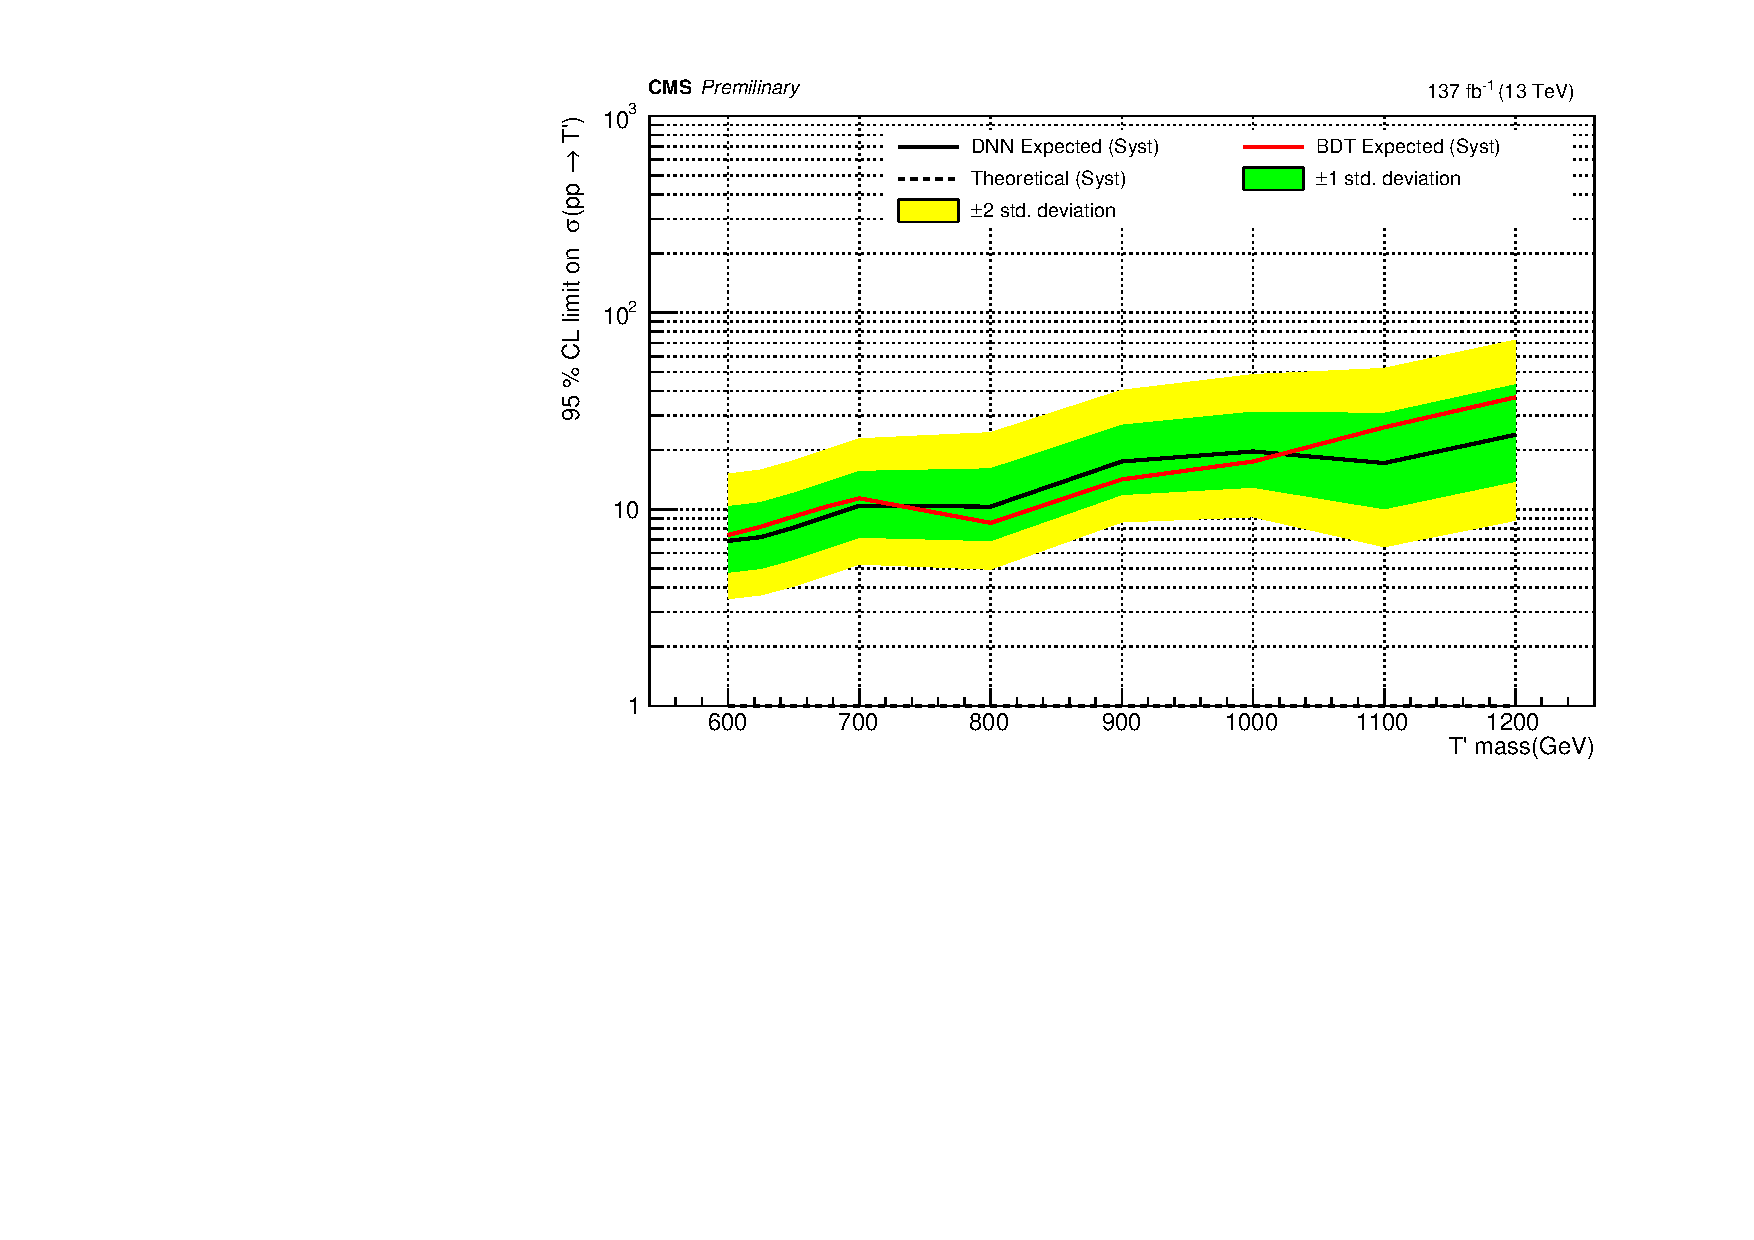
\includegraphics[scale=0.8]{figure_4/muALL_Plot_600-1200_.pdf}
    \caption{Expected 95\% CL limits for signal strength in the leptonic channel with comparison to the output of the BDT with $M_{T^'}$ $\in$ [600, 1200]GeV.}
    \label{fig:my_label_limit}
\end{figure}

The expected limit on the ${T^'}$ production cross-section are evaluated through \autoref{eq:1.1}, which is similar to the \autoref{eq:my_eqn_12}. The combined result together with the BDT comparison can be seen in the \autoref{fig:my_label_Comparision}.
\begin{equation} \label{eq:1.1}
    \sigma_{upper\ limit} = \mu_{upper\ limit} \times \sigma_{theory}
\end{equation}


\begin{figure}[H]
    \centering
    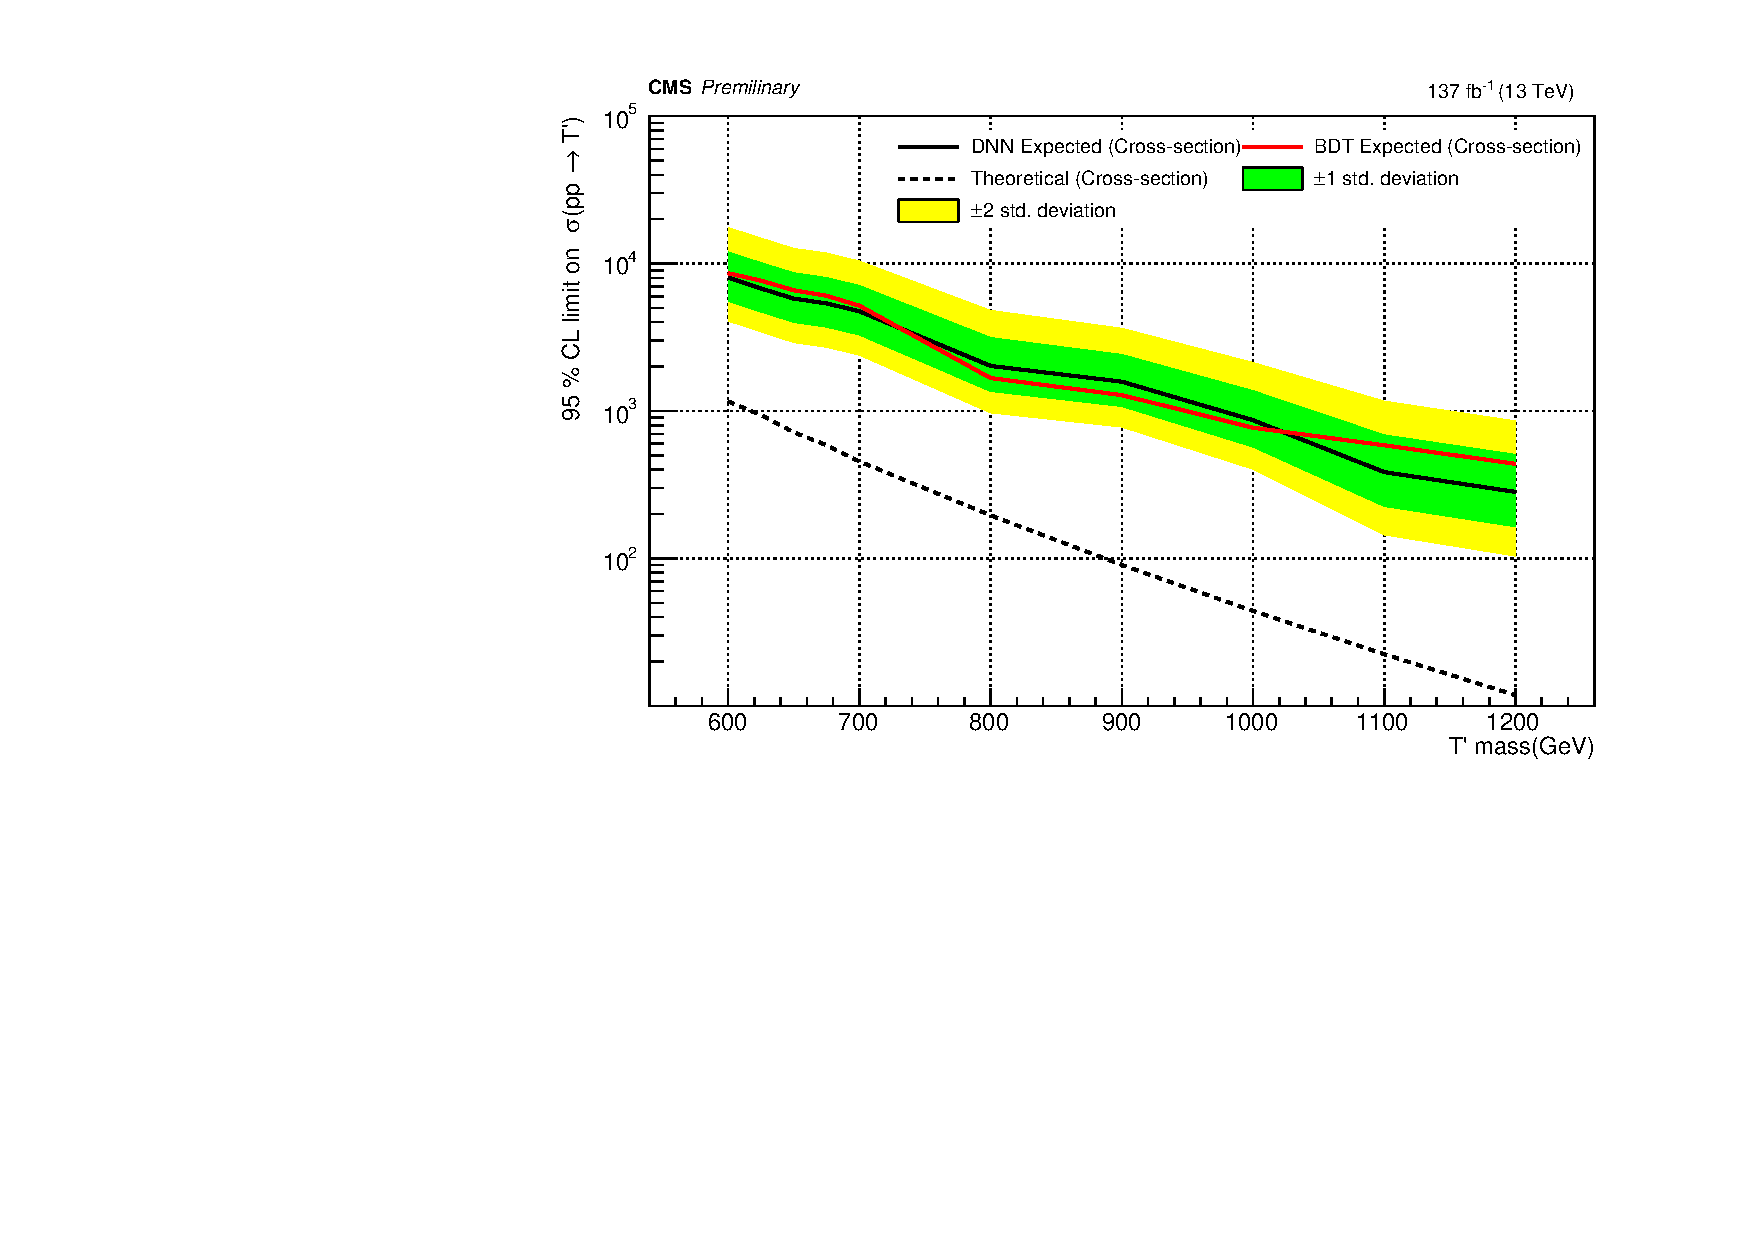
\includegraphics[scale=0.8]{figure_4/muALL_Plot_600-1200_with_cross_Section_comparision.pdf}
    \caption{Expected 95\% CL limits for $\sigma \times$ BR(H$\longrightarrow$$\gamma\gamma$)  in the leptonic channel with comaprision to the output of the BDT with $M_{T^'}$ $\in$ [600, 1200]GeV.}
    \label{fig:my_label_Comparision}
\end{figure}






% \url{https://cds.cern.ch/record/2789988?ln=en}
% \url{https://cdsweb.cern.ch/search?ln=en&cc=Theses&sc=1&p=VLQ&action_search=Search&op1=a&m1=a&p1=&f1=}
























% \section{Correlation between signal and background variable}
% A correlation function represents a measurement between the strength of a linear relationship between two quantitative variables. There are two types of correlation, positive correlation and negative correlation. Positive correlation represents a relationship between two variables in which both variables move in the same direction. This means when one variable increases while the other also increases and vice versa While negative correlation is a relationship where one variable increases as the other decreases, and vice versa. A correlation of 1 or +1 shows a perfect positive correlation, which means both the variables move in the same direction. A correlation of -1 shows a perfect negative correlation, which means as one variable goes down, the other goes up \cite{27}. Here for the comparison of the variables (given in \autoref{tab:my_label_1}) from two different datasets were calculated using Pearson Correlation Coefficient Formula, which is,
% \begin{equation}
%     r = \frac{n(\sum xy)- \sum x \sum y}{\sqrt{[n \sum x^2 - (\sum x)^2][n \sum y^2 - (\sum y)^2]}}
% \end{equation}
% Where,\\
% n = Quantity of Information \\
% $\sum x$ = Total of the First Variable Value \\
% $\sum y$ = Total of the Second Variable Value\\
% $\sum xy$ = Sum of the Product of first \& Second Value\\
% $\sum x^2$ = Sum of the Squares of the First Value\\
% $\sum y^2$ = Sum of the Squares of the Second Value\\

















\setcounter{equation}{0}
\setcounter{table}{0}
\setcounter{figure}{0}
%\baselineskip 24pt


    



